% -- \include{b2cexcl.tex}
% ======================================================================
\subsection{Exclusive CKM-favoured decays}
\label{slbdecays_b2cexcl}
% -------------------------------------------
This section is organized as follows: First, we present averages for
the decays $\bar B\to D^*\ell^-\bar\nu_\ell$ and $\bar B\to
D\ell^-\bar\nu_\ell$. In addition to the branching fractions, the CKM
element $|V_{cb}|$ is extracted. We then provide
averages for the inclusive branching fractions $\cbf(\bar B\to
D^{(*)}\pi \ell^-\bar\nu_\ell)$ and for $B$ semileptonic decays into
orbitally-excited $P$-wave charm mesons ($D^{**}$). As the $D^{**}$
branching fraction is poorly known, we report the averages for the products 
$\cbf(B^-\to D^{**}(D^{(*)}\pi)\ell^-\bar\nu_\ell)\times
\cbf(D^{**}\to D^{(*)}\pi)$.

%===================================================================
% D and D* 
%===================================================================

\mysubsubsection{$\bar B\to D^*\ell^-\bar\nu_\ell$}
\label{slbdecays_dstarlnu}

The kinematics of the decay $\bar B\to D^*\ell^-\bar\nu_\ell$ are
described by the form factor $\eta_\mathrm{EW}{\cal F}(w)$, where
$\eta_{EW}$ is a known electro-weak correction factor and $w$ is the
product of the $B$ and $D^*$ meson 4-velocities, $w=v_B\cdot
v_{D^*}$. Most experiments use the parameterization of Caprini,
Lellouch and Neubert (CLN) to describe the shape and normalization of
$\eta_\mathrm{EW}{\cal F}(w)$ by four quantities:
$\eta_\mathrm{EW}{\cal F}(1)\vcb$, $\rho^2$, $R_1(1)$ and
$R_2(1)$~\cite{CLN}. Our main average and the determination of $\vcb$
are based on this parameterization.

We use the measurements of these form factor parameters shown in
Table~\ref{tab:vcbf1} and rescale them to the latest values of the
input parameters (mainly branching fractions of charmed
mesons)~\cite{HFAG_sl:inputparams}. Most of the measurements in
Table~\ref{tab:vcbf1} are based exclusively on the decay $\bar B^0\to
D^{*+}\ell^-\bar\nu_\ell$. Some
measurements~\cite{Adam:2002uw,Aubert:2009_1} are sensitive also to
$B^-\to D^{*0}\ell^-\bar\nu_\ell$ and one
measurement~\cite{Aubert:2009_3} is based exclusively on the decay
$B^-\to D^{*0}\ell^-\bar\nu_\ell$. Our analysis thus assumes isospin
symmetry.
% ----------------------------------------------------------------------
\begin{table}[!htb]
\caption{Measurements of the Caprini, Lellouch and Neubert
  (CLN)~\cite{CLN} form factor parameters in $\bar B\to
  D^*\ell^-\bar\nu_\ell$ before and after rescaling. Most analyses
  (except \cite{Dungel:2010uk,Aubert:2006mb}) measure only
  $\eta_\mathrm{EW}{\cal F}(1)\vcb$, and $\rho^2$, so only these two
  parameters are shown here. The average is the result of a
  4-dimensional fit to the rescaled measurements of
  $\eta_\mathrm{EW}{\cal F}(1)\vcb$, $\rho^2$, $R_1(1)$ and
  $R_2(1)$ -- see the text for more details. The $\chi^2$~value of the
  combination is 30.0 for 23 degrees of freedom (CL=$15.0\%$).}
\begin{center}
\resizebox{0.99\textwidth}{!}{
\begin{tabular}{|l|c|c|}
  \hline
  Experiment
  & $\eta_\mathrm{EW}{\cal F}(1)\vcb [10^{-3}]$ (rescaled)
  & $\rho^2$ (rescaled)\\
  & $\eta_\mathrm{EW}{\cal F}(1)\vcb [10^{-3}]$ (published)
  & $\rho^2$ (published)\\
  \hline\hline
  ALEPH~\cite{Buskulic:1996yq}
  & $31.23\pm 1.80_{\rm stat}\pm 1.30_{\rm syst}$
  & $0.493\pm 0.228_{\rm stat}\pm 0.144_{\rm syst}$\\
  & $31.9\pm 1.8_{\rm stat}\pm 1.9_{\rm syst}$
  & $0.37\pm 0.26_{\rm stat}\pm 0.14_{\rm syst}$\\
  \hline
  CLEO~\cite{Adam:2002uw}
  & $39.94\pm 1.23_{\rm stat}\pm 1.62_{\rm syst}$
  & $1.367\pm 0.085_{\rm stat}\pm 0.086_{\rm syst}$\\
  & $43.1\pm 1.3_{\rm stat}\pm 1.8_{\rm syst}$
  & $1.61\pm 0.09_{\rm stat}\pm 0.21_{\rm syst}$\\
  \hline
  OPAL excl~\cite{Abbiendi:2000hk}
  & $36.50\pm 1.60_{\rm stat}\pm 1.49_{\rm syst}$
  & $1.234\pm 0.212_{\rm stat}\pm 0.145_{\rm syst}$\\
  & $36.8\pm 1.6_{\rm stat}\pm 2.0_{\rm syst}$
  & $1.31\pm 0.21_{\rm stat}\pm 0.16_{\rm syst}$\\
  \hline
  OPAL partial reco~\cite{Abbiendi:2000hk}
  & $37.14\pm 1.19_{\rm stat}\pm 2.36_{\rm syst}$
  & $1.152\pm 0.145_{\rm stat}\pm 0.294_{\rm syst}$\\
  & $37.5\pm 1.2_{\rm stat}\pm 2.5_{\rm syst}$
  & $1.12\pm 0.14_{\rm stat}\pm 0.29_{\rm syst}$\\
  \hline
  DELPHI partial reco~\cite{Abreu:2001ic}
  & $35.32\pm 1.40_{\rm stat}\pm 2.33_{\rm syst}$
  & $1.174\pm 0.126_{\rm stat} \pm 0.377_{\rm syst}$\\
  & $35.5\pm 1.4_{\rm stat}\ {}^{+2.3}_{-2.4}{}_{\rm syst}$
  & $1.34\pm 0.14_{\rm stat}\ {}^{+0.24}_{-0.22}{}_{\rm syst}$\\
  \hline
  DELPHI excl~\cite{Abdallah:2004rz}
  & $36.10\pm 1.70_{\rm stat}\pm 1.97_{\rm syst}$
  & $1.081\pm 0.142_{\rm stat} \pm 0.152_{\rm syst}$\\
  & $39.2\pm 1.8_{\rm stat}\pm 2.3_{\rm syst}$
  & $1.32\pm 0.15_{\rm stat}\pm 0.33_{\rm syst}$\\
  \hline
  \belle~\cite{Dungel:2010uk}
  & $34.60\pm 0.17_{\rm stat}\pm 1.02_{\rm syst}$
  & $1.212\pm 0.034_{\rm stat}\pm 0.009_{\rm syst}$\\
  & $34.6\pm 0.2_{\rm stat}\pm 1.0_{\rm syst}$
  & $1.214\pm 0.034_{\rm stat} \pm 0.009_{\rm syst}$\\
  \hline
  \babar\ excl~\cite{Aubert:2006mb}
  & $33.94\pm 0.30_{\rm stat}\pm 0.99_{\rm syst}$
  & $1.185\pm 0.048_{\rm stat}\pm 0.029_{\rm syst}$\\
  & $34.7\pm 0.3_{\rm stat}\pm 1.1_{\rm syst}$
  & $1.18\pm 0.05_{\rm stat}\pm 0.03_{\rm syst}$\\
  \hline
  \babar\ $D^{*0}$~\cite{Aubert:2009_3}
  & $35.22\pm 0.59_{\rm stat}\pm 1.33_{\rm syst}$
  & $1.128\pm 0.058_{\rm stat}\pm 0.055_{\rm syst}$\\
  & $35.9\pm 0.6_{\rm stat}\pm 1.4_{\rm syst}$
  & $1.16\pm 0.06_{\rm stat}\pm 0.08_{\rm syst}$\\
  \hline
  \babar\ global fit~\cite{Aubert:2009_1}
  & $35.76\pm 0.20_{\rm stat}\pm 1.10_{\rm syst}$
  & $1.193\pm 0.020_{\rm stat}\pm 0.061_{\rm syst}$\\
  & $35.7\pm 0.2_{\rm stat}\pm 1.2_{\rm syst}$
  & $1.21\pm 0.02_{\rm stat}\pm 0.07_{\rm syst}$\\
  \hline
  {\bf Average}
  & \mathversion{bold} $35.81\pm 0.11_{\rm stat}\pm 0.44_{\rm syst}$ &
  \mathversion{bold} $1.207\pm 0.015_{\rm stat}\pm 0.021_{\rm syst}$\\
  \hline 
\end{tabular}
}
\end{center}
\label{tab:vcbf1}
\end{table}
% ----------------------------------------------------------------------


In the next step, we perform a four-dimensional fit of the parameters
$\eta_\mathrm{EW}{\cal F}(1)\vcb$, $\rho^2$, $R_1(1)$ and $R_2(1)$
using the rescaled measurements and taking into account correlated
statistical and systematic uncertainties. Only two measurements
constrain all four parameters~\cite{Dungel:2010uk,Aubert:2006mb}, the remaining
measurements determine only the normalization $\eta_\mathrm{EW}{\cal
  F}(1)\vcb$ and the slope $\rho^2$. The result of the fit is
\begin{eqnarray}
  \eta_\mathrm{EW}{\cal F}(1)\vcb & = & (35.81\pm 0.45)\times
  10^{-3}~, \label{eq:vcbf1} \\
  \rho^2 & = & 1.207\pm 0.026~,\\
  R_1(1) & = & 1.406\pm 0.033~, \label{eq:r1} \\
  R_2(1) & = & 0.853\pm 0.020~, \label{eq:r2}
\end{eqnarray}
and the correlation coefficients are
\begin{eqnarray}
  \rho_{\eta_\mathrm{EW}{\cal F}(1)\vcb,\rho^2} & = & 0.323~,\\
  \rho_{\eta_\mathrm{EW}{\cal F}(1)\vcb,R_1(1)} & = & -0.108~,\\
  \rho_{\eta_\mathrm{EW}{\cal F}(1)\vcb,R_2(1)} & = & -0.063~,\\
  \rho_{\rho^2,R_1(1)} & = & 0.568~,\\
  \rho_{\rho^2,R_2(1)} & = & -0.809~,\\
  \rho_{R_1(1),R_2(1)} & = & -0.758~.
\end{eqnarray}
The uncertainties and correlations quoted here include both
statistical and systematic contributions. The $\chi^2$ of the fit is
30.0 for 23 degrees of freedom, which corresponds to a confidence
level of 15.0\%. An illustration of this fit result is given in
Fig.~\ref{fig:vcbf1}.
\begin{figure}[!ht]
  \begin{center}
  \unitlength 1.0cm % coordinates in cm
  \begin{picture}(14.,8.0)
    \put(  8.0,
    -0.2){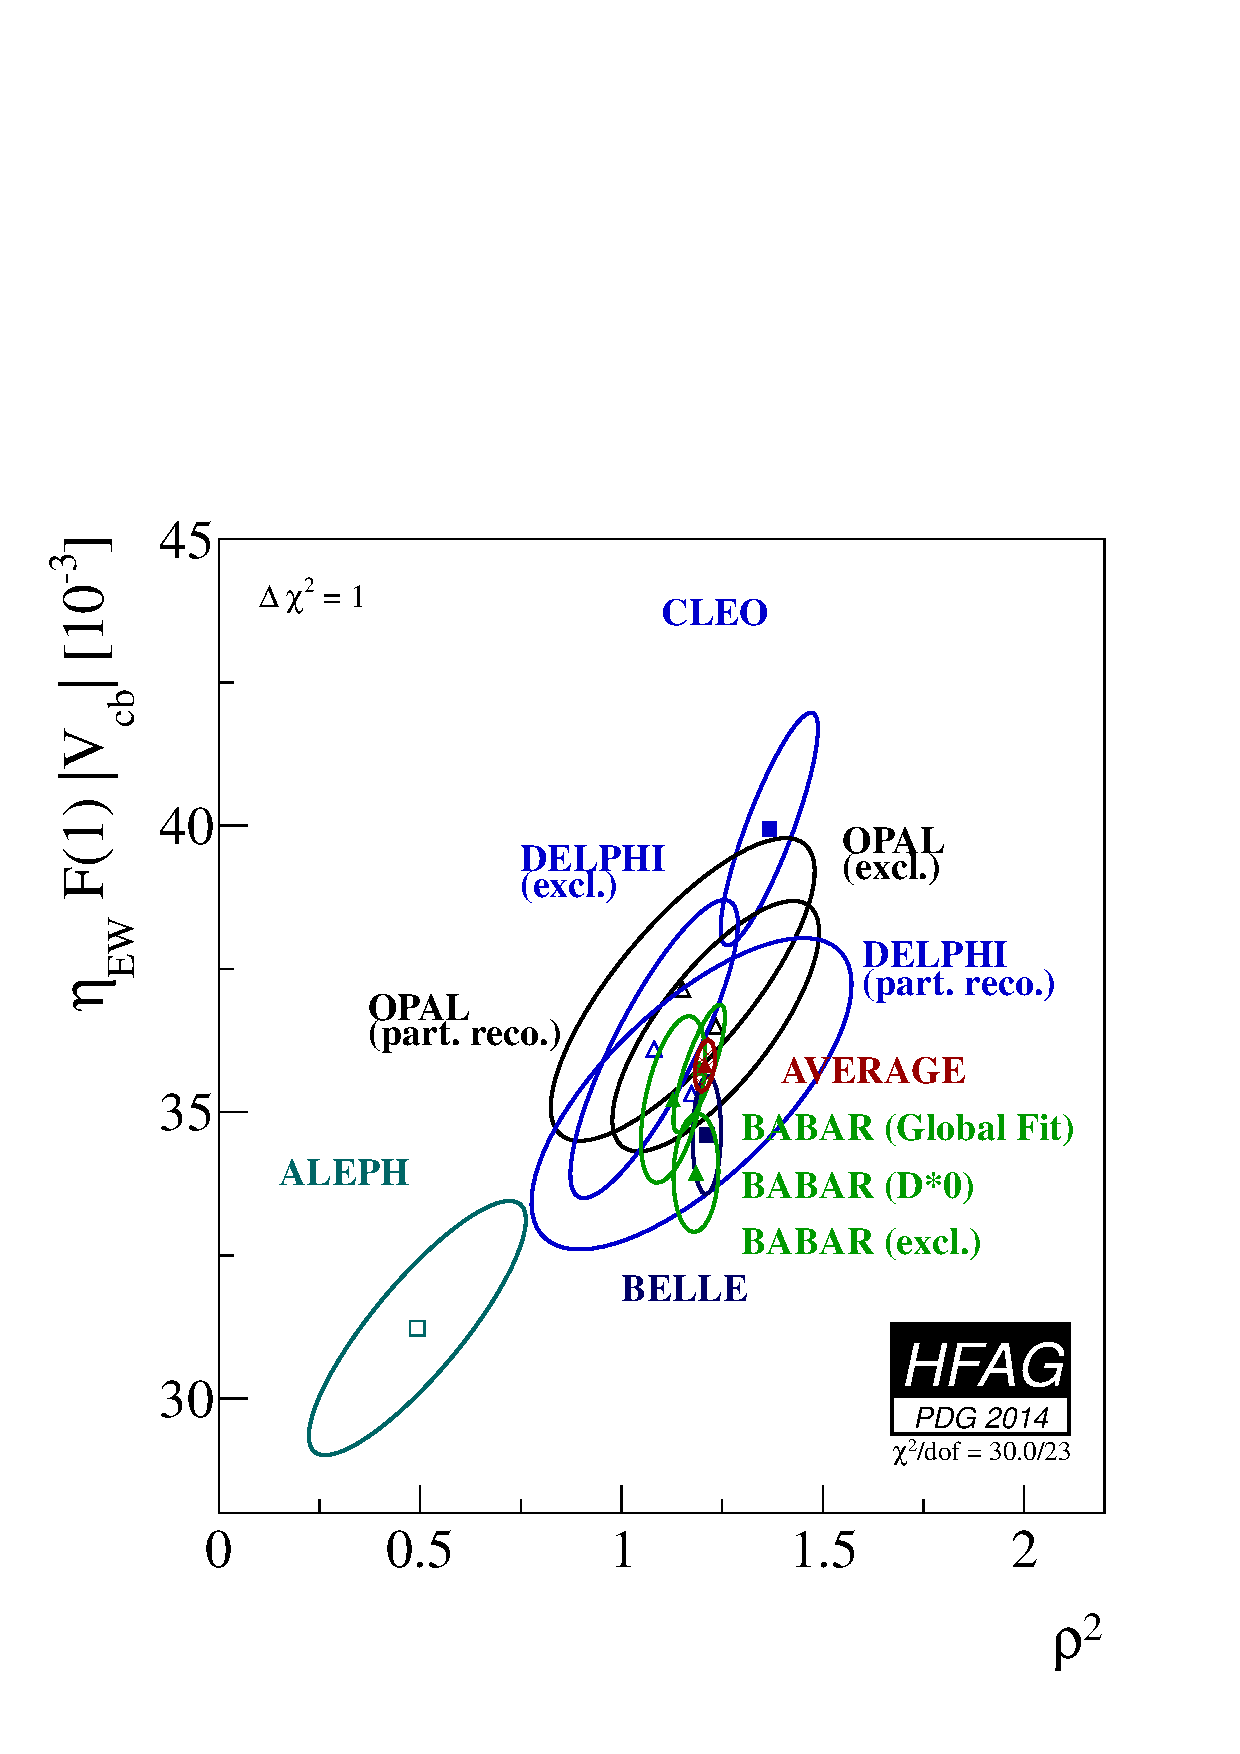
\includegraphics[width=8.0cm]{figures/slb/vcbf1_vs_rho2.pdf}
    }
    \put( -0.5,
    0.0){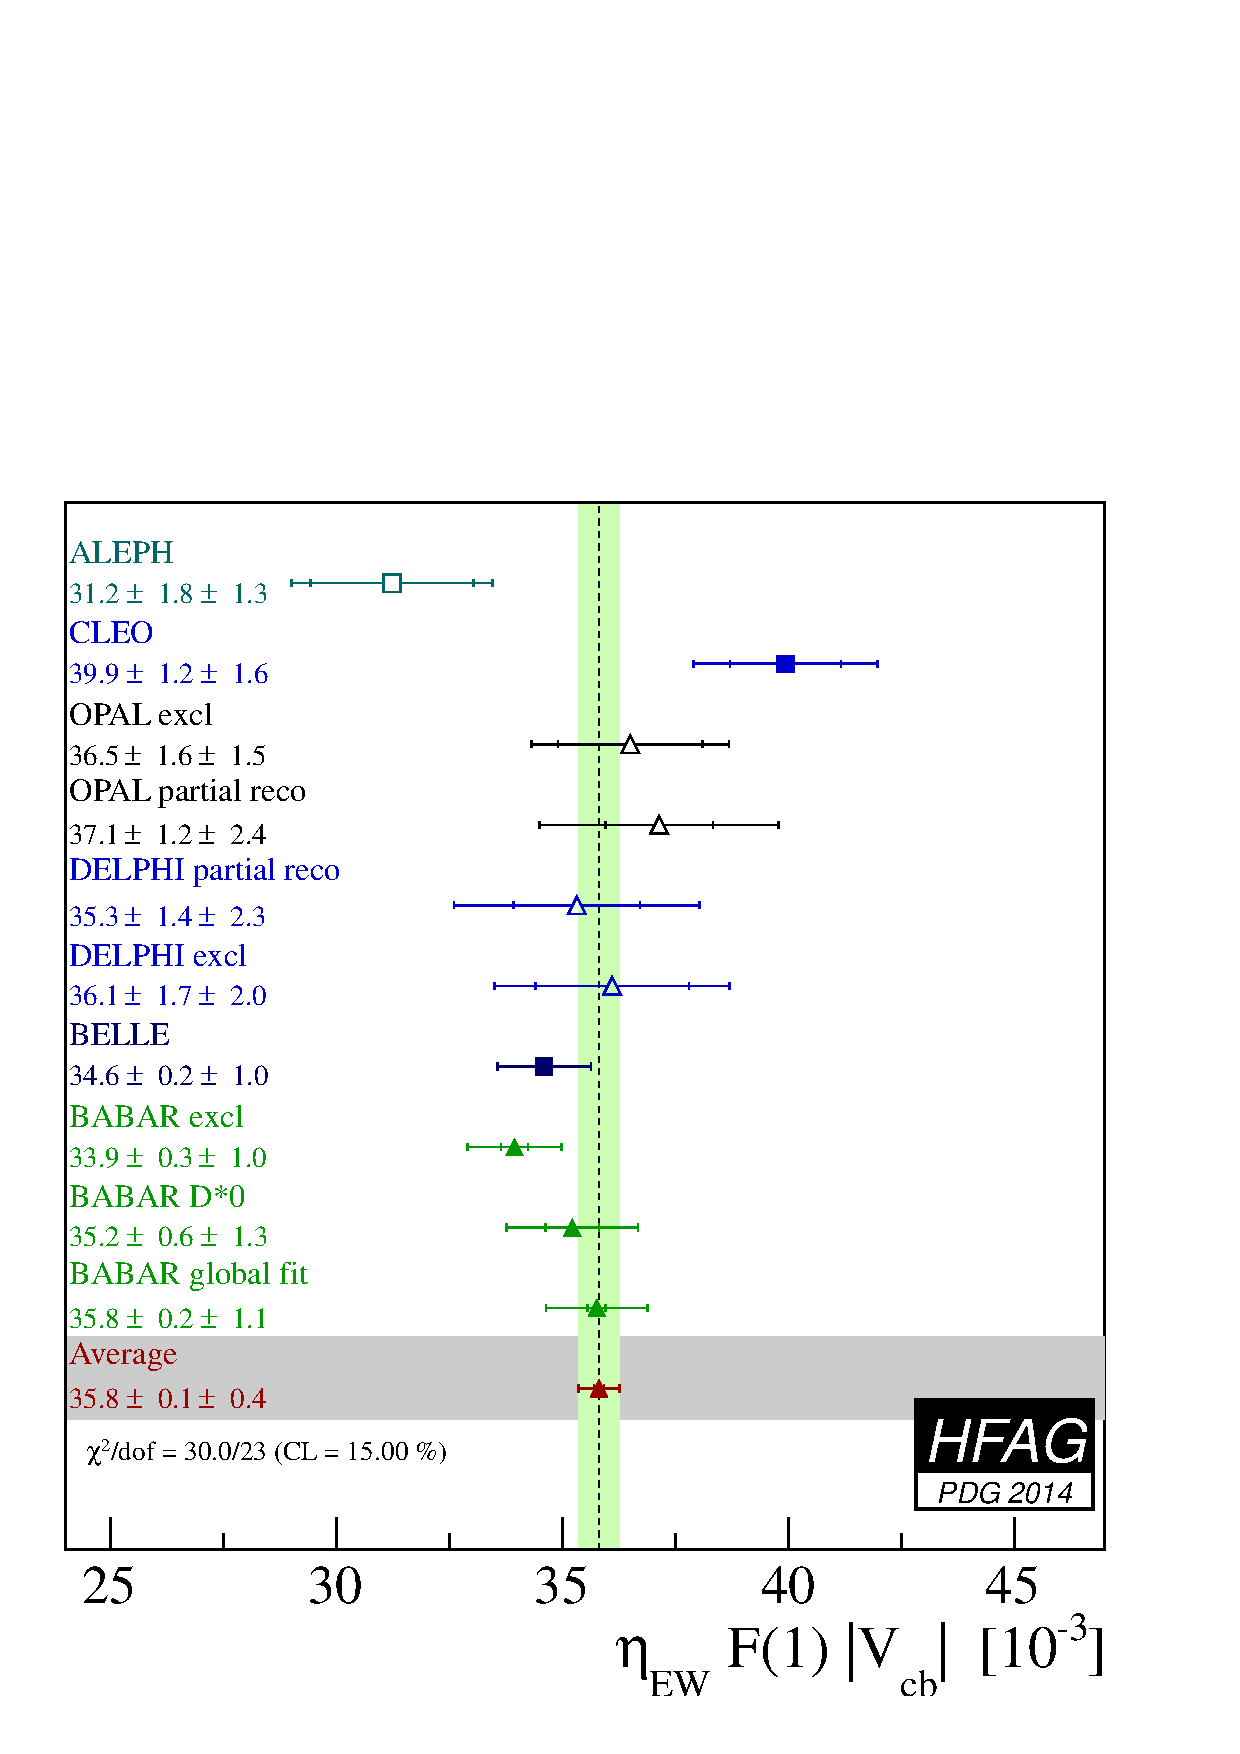
\includegraphics[width=7.5cm]{figures/slb/vcbf1.pdf}
    }
    \put(  5.5,  6.8){{\large\bf a)}}  
    \put( 14.4,  6.8){{\large\bf b)}}
  \end{picture}
  \caption{(a) Illustration of the $\eta_\mathrm{EW}{\cal F}(1)\vcb$
      average. (b) Illustration of the $\eta_\mathrm{EW}{\cal
        F}(1)\vcb$ vs.\ $\rho^2$ average. The error ellipses
      correspond  to $\Delta\chi^2 = 1$ (CL=39\%).} \label{fig:vcbf1}
  \end{center}
\end{figure}

Using the lastest update from the FNAL/MILC
group~\cite{Bailey:2014tva}, the form factor normalization
$\eta_\mathrm{EW}{\cal F}(1)$ is
\begin{equation}
  \eta_\mathrm{EW}{\cal F}(1) = 0.920\pm 0.014~,
\end{equation}
which results in the following determination of $\vcb$ from
Eq.~\ref{eq:vcbf1},
\begin{equation}
  \vcb = (38.94\pm 0.49_{\rm exp}\pm 0.58_{\rm th})\times
  10^{-3}~, \label{eq:vcbdstar}
\end{equation}
where the first uncertainty is experimental and the second error is
theoretical (lattice QCD calculation and electro-weak correction).

From each rescaled measurement in Table~\ref{tab:vcbf1}, we
calculate the $\bar B\to D^*\ell^-\bar\nu_\ell$ form factor
$\eta_\mathrm{EW}{\cal F}(w)$ and, by numerical integration, the
branching ratio of the decay $\bar B^0\to
D^{*+}\ell^-\bar\nu_\ell$. For measurements which do not determine the
parameters $R_1(1)$ and $R_2(1)$ we assume the average
values~Eqs.~\ref{eq:r1} and \ref{eq:r2}. The results are quoted in
Table~\ref{tab:dstarlnu}. The branching ratio found for the average
values of $\eta_\mathrm{EW}{\cal F}(1)\vcb$, $\rho^2$, $R_1(1)$ and
$R_2(1)$ is
\begin{equation}
  \cbf(\BzbDstarlnu)=(4.93\pm 0.11)\%~.
\end{equation}

To test isospin symmetry, we have performed a simple 1-dimensional
average of measurements sensitive to the decay $B^-\to
D^{*0}\ell^-\bar\nu_\ell$ only, which is shown in
Table~\ref{tab:dstar0lnu}. Fig.~\ref{fig:brdsl} illustrates our two
averages of $\bar B\to D^*\ell^-\bar\nu_\ell$.
% ----------------------------------------------------------------------
\begin{table}[!htb]
\caption{$\BzbDstarlnu$ branching fractions calculated from the
  rescaled measurements in Table~\ref{tab:vcbf1}, asumming the CLN
  parameterization of the form factor~\cite{CLN}. The branching ratios
  published in Refs.~\cite{Aubert:2009_3,Aubert:2009_1} have been
  rescaled by the factor $\tau(B^0)/\tau(B^+)$. While the fit assumes
  isospin symmetry, most measurements included here use only the decay
  $\BzbDstarlnu$.}
\begin{center} 
\resizebox{0.99\textwidth}{!}{
\begin{tabular}{|l|c|c|}\hline
  Experiment & $\cbf(\BzbDstarlnu)$ [\%] (calculated) &
  $\cbf(\BzbDstarlnu)$ [\%] (published)\\
  \hline\hline
  ALEPH~\hfill\cite{Buskulic:1996yq}
  & $5.35\pm 0.25_{\rm stat} \pm 0.31_{\rm syst}$
  & $5.53\pm 0.26_{\rm stat} \pm 0.52_{\rm syst}$\\
  CLEO~\hfill\cite{Adam:2002uw}
  & $5.62\pm 0.18_{\rm stat} \pm 0.26_{\rm syst}$
  & $6.09\pm 0.19_{\rm stat} \pm 0.40_{\rm syst}$\\
  OPAL excl~\hfill\cite{Abbiendi:2000hk}
  & $5.05\pm 0.19_{\rm stat} \pm 0.42_{\rm syst}$
  & $5.11\pm 0.19_{\rm stat} \pm 0.49_{\rm syst}$\\
  OPAL partial reco~\hfill\cite{Abbiendi:2000hk}
  & $5.46\pm 0.25_{\rm stat} \pm 0.52_{\rm syst}$
  & $5.92\pm 0.27_{\rm stat} \pm 0.68_{\rm syst}$\\
  DELPHI partial reco~\hfill\cite{Abreu:2001ic}
  & $4.88\pm 0.13_{\rm stat} \pm 0.72_{\rm syst}$
  & $4.70\pm 0.13_{\rm stat} \ {}^{+0.36}_{-0.31}\ {}_{\rm syst}$\\
  DELPHI excl~\hfill\cite{Abdallah:2004rz}
  & $5.35\pm 0.20_{\rm stat} \pm 0.37_{\rm syst}$
  & $5.90\pm 0.22_{\rm stat} \pm 0.50_{\rm syst}$\\
  \belle~\hfill\cite{Dungel:2010uk}
  & $4.56\pm 0.03_{\rm stat} \pm 0.26_{\rm syst}$
  & $4.58\pm 0.03_{\rm stat} \pm 0.26_{\rm syst}$\\
  \babar\ excl~\hfill\cite{Aubert:2006mb}
  & $4.54\pm 0.04_{\rm stat}\pm 0.25_{\rm syst}$
  & $4.69\pm 0.04_{\rm stat} \pm 0.34_{\rm syst}$\\
  \babar\ $D^{*0}$~\hfill\cite{Aubert:2009_3}
  & $4.97\pm 0.07_{\rm stat}\pm 0.34_{\rm syst}$
  & $5.15\pm 0.07_{\rm stat} \pm 0.38_{\rm syst}$\\
  \babar\ global fit~\hfill\cite{Aubert:2009_1}
  & $4.95\pm 0.02_{\rm stat}\pm 0.20_{\rm syst}$
  & $5.00\pm 0.02_{\rm stat} \pm 0.19_{\rm syst}$\\
  \hline 
  {\bf Average} & \mathversion{bold}$4.93\pm 0.01_{\rm stat}\pm
  0.11_{\rm syst}$ & \mathversion{bold}$\chi^2/\dof = 30.0/23$ (CL=$15.0\%$)\\
  \hline 
\end{tabular}
}
\end{center}
\label{tab:dstarlnu}
\end{table}
% ----------------------------------------------------------------------

% ----------------------------------------------------------------------0
\begin{table}[!htb]
\caption{Average of the $B^-\to D^{*0}\ell^-\bar\nu_\ell$ branching
  fraction measurements. This fit uses only measurements of $B^-\to
  D^{*0}\ell^-\bar\nu_\ell$.}
\begin{center}
\begin{tabular}{|l|c|c|}
  \hline
  Experiment & $\cbf(B^-\to D^{*0}\ell^-\bar\nu_\ell)$ [\%] (rescaled) &
  $\cbf(B^-\to D^{*0}\ell^-\bar\nu_\ell)$ [\%] (published)\\
  \hline \hline
  CLEO~\hfill\cite{Adam:2002uw}
  & $6.61\pm 0.20_{\rm stat}\pm 0.39_{\rm syst}$
  & $6.50\pm 0.20_{\rm stat}\pm 0.43_{\rm syst}$\\
  \babar tagged~\hfill\cite{Aubert:vcbExcl}
  & $5.72\pm 0.15_{\rm stat}\pm 0.30_{\rm syst}$
  & $5.83\pm 0.15_{\rm stat}\pm0.30_{\rm syst}$\\
  \babar~\hfill\cite{Aubert:2009_3}
  & $5.35\pm0.08_{\rm stat}\pm 0.40_{\rm syst}$
  & $5.56\pm0.08_{\rm stat} \pm0.41_{\rm syst}$\\
  \babar~\hfill\cite{Aubert:2009_1}
  & $5.43\pm 0.02_{\rm stat}\pm 0.21_{\rm syst}$
  & $5.40\pm 0.02_{\rm stat}\pm 0.21_{\rm syst}$\\
  \hline
  {\bf Average} & \mathversion{bold}$5.70\pm 0.02_{\rm stat}\pm
  0.19_{\rm syst}$ & \mathversion{bold}$\chi^2/\dof = 9.1/3$ (CL=$2.8\%$)\\
  \hline 
\end{tabular}
\end{center}
\label{tab:dstar0lnu}
\end{table}
% ----------------------------------------------------------------------

\begin{figure}[!ht]
  \begin{center}
  \unitlength1.0cm % coordinates in cm
  \begin{picture}(14.,8.0)  %ys(25.,6.0)
    \put( -0.5, 0.0){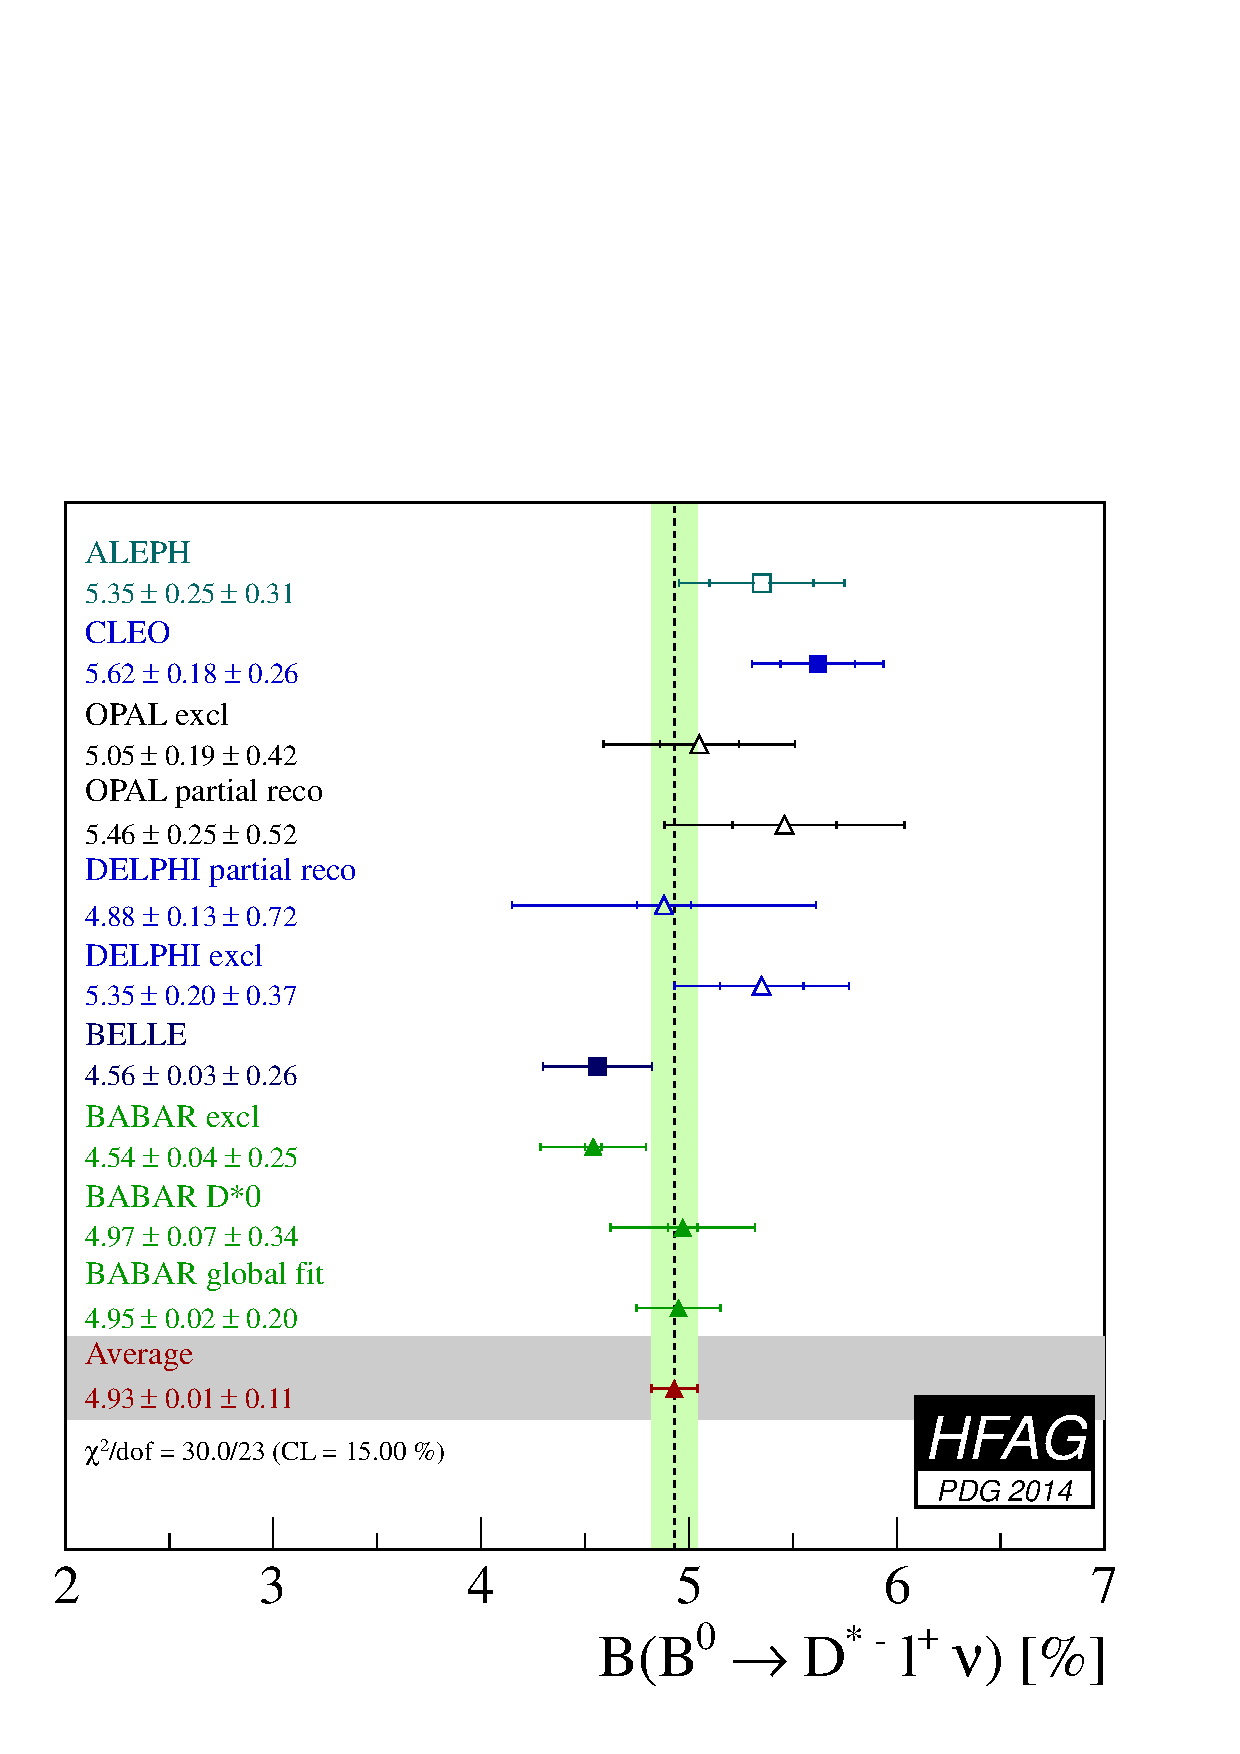
\includegraphics[width=7.5cm]{figures/slb/br_dsl_iso.pdf}
    }
    \put(  8.0, 0.0){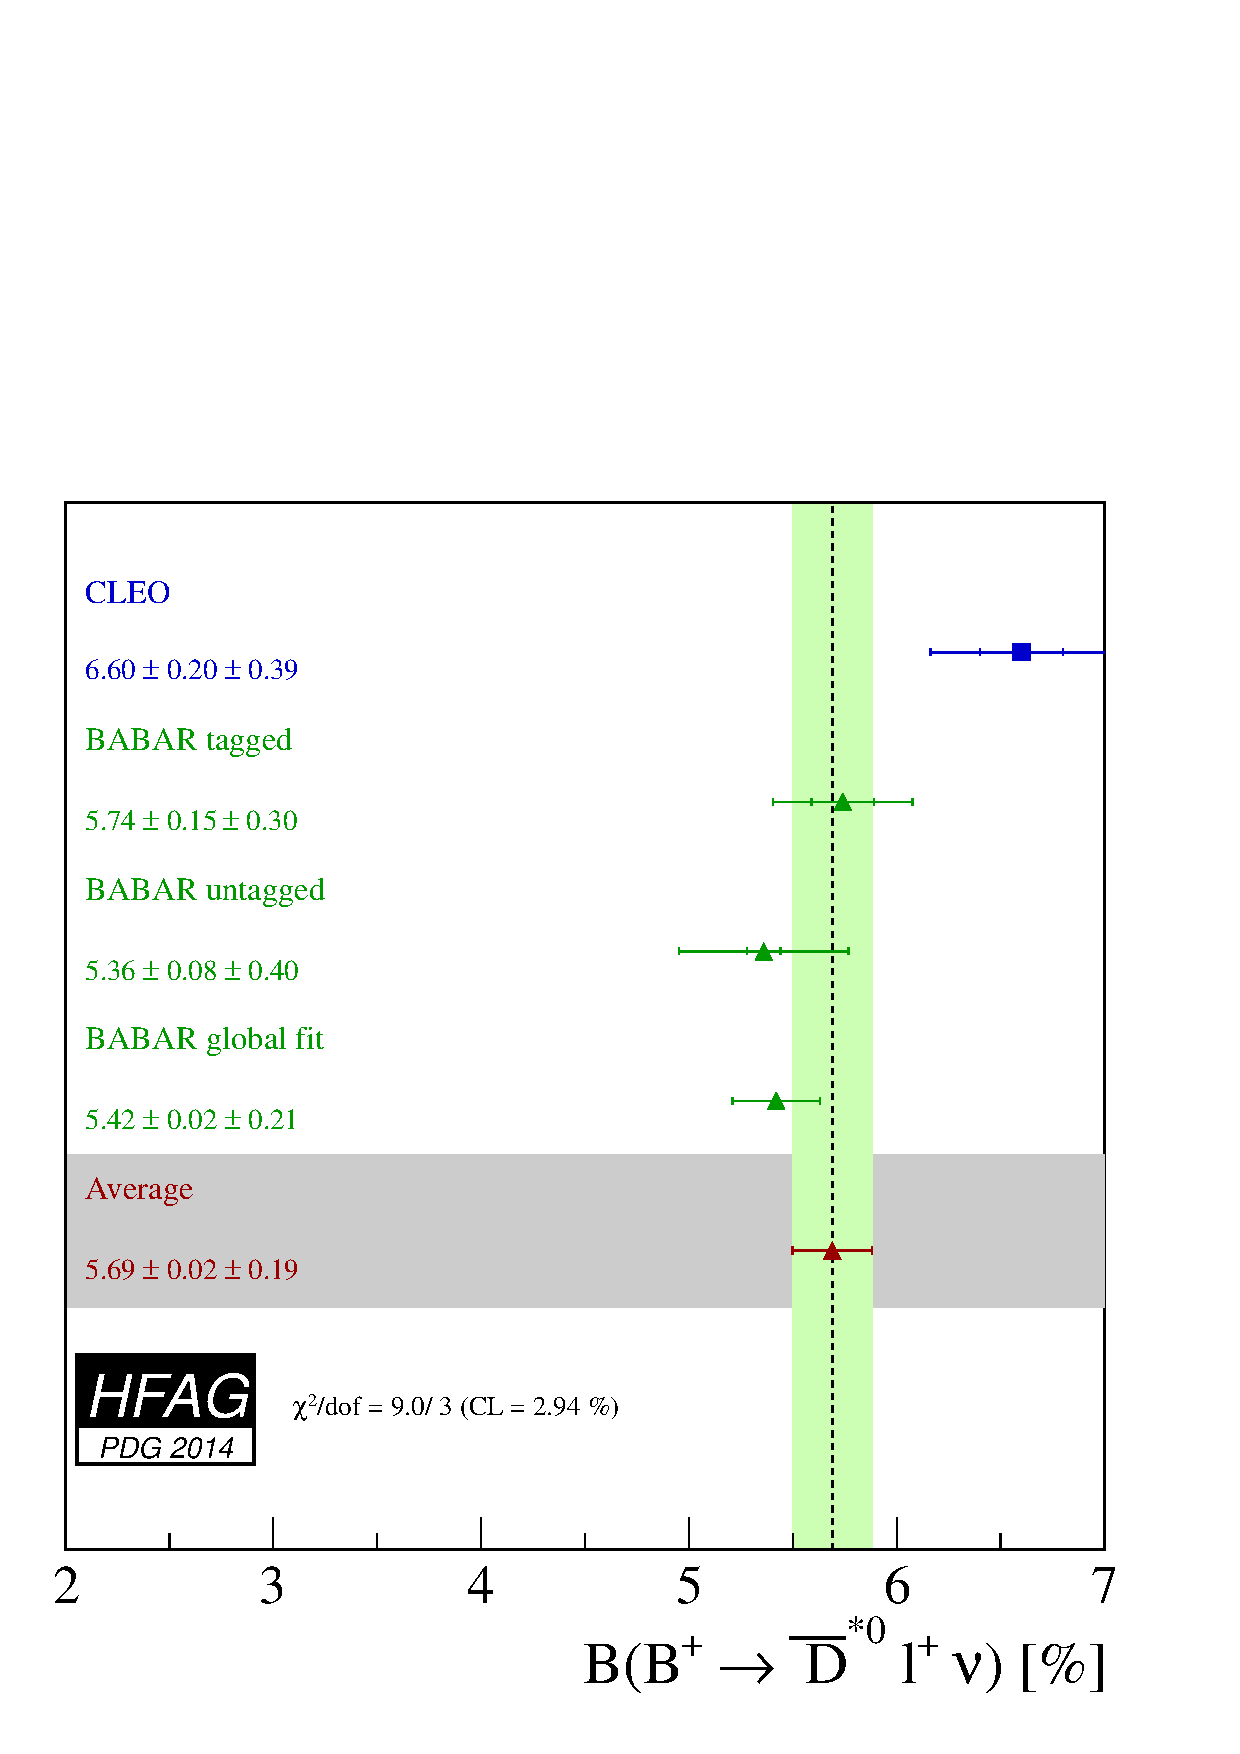
\includegraphics[width=7.5cm]{figures/slb/br_ds0l.pdf}
    }
    \put(  5.5, 6.8){{\large\bf a)}}
    \put( 14.0, 6.8){{\large\bf b)}}
  \end{picture}
  \caption{(a) Average branching fractions of exclusive semileptonic
    $B$ decays $\bar B\to D^*\ell^-\bar\nu_\ell$: (a) $\BzbDstarlnu$
    (Table~\ref{tab:dstarlnu}) and (b) $B^-\to
    D^{*0}\ell^-\bar\nu_\ell$ (Table~\ref{tab:dstar0lnu}).} \label{fig:brdsl}
  \end{center}
\end{figure}

\mysubsubsection{$\bar B\to D\ell^-\bar\nu_\ell$}
\label{slbdecays_dlnu}

The relevant form factor for the decay $\bar B\to D\ell^-\bar\nu_\ell$
is $\eta_\mathrm{EW}{\cal G}(w)$, which in CLN~\cite{CLN} is described
by only two parameters: the normalization $\eta_\mathrm{EW}{\cal
  G}(1)\vcb$ and the slope $\rho^2$.

We use the measurements of these two form factor parameters shown in
Table~\ref{tab:vcbg1} and correct them to match the latest values of
the input parameters~\cite{HFAG_sl:inputparams}. These measurements
are sensitive to both isospin states ($\BzbDplnu$ and $B^-\to
D^0\ell^-\bar\nu_\ell$). So, isospin symmetry is assumed in the analysis.
\begin{table}[!htb]
\caption{Measurements of $\bar B\to D\ell^-\bar\nu_\ell$ in the
  parameterization of Caprini, Lellouch and Neubert
  (CLN)~\cite{CLN}. The average is the result of a 2-dimensional fit
  to the rescaled measurements of ${\cal G}(1)\vcb$ and $\rho^2$. The
  $\chi^2$~value of the combination is 0.5 for 8 degrees of freedom
  (CL=$100.0\%$). The total correlation between the average ${\cal G}(1)\vcb$
  and $\rho^2$ is 0.83.}
\begin{center}
\begin{tabular}{|l|c|c|}
  \hline
  Experiment
  & ${\cal G}(1)\vcb$ [10$^{-3}$] (rescaled)
  & $\rho^2$ (rescaled)\\
  & ${\cal G}(1)\vcb$ [10$^{-3}$] (published)
  & $\rho^2$ (published)\\
  \hline \hline
  ALEPH~\hfill\cite{Buskulic:1996yq}
  & $38.89\pm 11.80_{\rm stat}\pm 6.09_{\rm syst}$
  & $0.951\pm 0.980_{\rm stat}\pm 0.357_{\rm syst}$\\
  & $31.1\pm 9.9_{\rm stat}\pm 8.6_{\rm syst}$
  & $0.70\pm 0.98_{\rm stat}\pm 0.50_{\rm syst}$\\
  \hline
  CLEO~\hfill\cite{Bartelt:1998dq}
  & $44.90\pm 5.97_{\rm stat}\pm 3.30_{\rm syst}$
  & $1.270\pm 0.250_{\rm stat}\pm 0.140_{\rm syst}$\\
  & $44.8\pm 6.1_{\rm stat}\pm 3.7_{\rm syst}$
  & $1.30\pm 0.27_{\rm stat}\pm 0.14_{\rm syst}$\\
  \hline
  \belle~\hfill\cite{Abe:2001yf}
  & $40.84\pm 4.37_{\rm stat}\pm 5.17_{\rm syst}$
  & $1.120\pm 0.220_{\rm stat}\pm 0.140_{\rm syst}$\\
  & $41.1\pm 4.4_{\rm stat}\pm 5.1_{\rm syst}$
  & $1.12\pm 0.22_{\rm stat}\pm 0.14_{\rm syst}$\\
  \hline
  \babar global fit~\hfill\cite{Aubert:2009_1}
  & $43.42\pm 0.81_{\rm stat}\pm 2.08_{\rm syst}$
  & $1.204\pm 0.040_{\rm stat}\pm 0.057_{\rm syst}$\\
  & $43.1\pm 0.8_{\rm stat}\pm 2.3_{\rm syst}$
  & $1.20\pm 0.04_{\rm stat}\pm 0.07_{\rm syst}$\\
  \hline
  \babar tagged~\hfill\cite{Aubert:2009_2}
  & $42.45\pm 1.88_{\rm stat}\pm 1.05_{\rm syst}$
  & $1.180\pm 0.089_{\rm stat}\pm 0.051_{\rm syst}$\\
  & $42.3\pm 1.9_{\rm stat}\pm 1.0_{\rm syst}$
  & $1.20\pm 0.09_{\rm stat}\pm 0.04_{\rm syst}$\\
  \hline 
  {\bf Average }
  & \mathversion{bold}$42.64\pm 0.72_{\rm stat}\pm 1.35_{\rm syst}$
  & \mathversion{bold}$1.186\pm 0.036_{\rm stat}\pm 0.041_{\rm syst}$\\
  \hline 
\end{tabular}
\end{center}
\label{tab:vcbg1}
\end{table}


The form factor parameters are extracted by a two-dimensional fit to
the rescaled measurements of $\eta_\mathrm{EW}{\cal G}(1)\vcb$ and
$\rho^2$ taking into account correlated statistical and systematic
uncertainties. The result of the fit reads
\begin{eqnarray}
  \eta_\mathrm{EW}{\cal G}(1)\vcb & = & (42.65\pm 1.53)\times
  10^{-3}~, \label{eq:vcbg1} \\
  \rho^2 & = & 1.185 \pm 0.054~,
\end{eqnarray}
with a correlation of
\begin{equation}
  \rho_{\eta_\mathrm{EW}{\cal G}(1)\vcb,\rho^2} = 0.824~.
\end{equation}
The uncertainties and the correlation coefficient include both
statistical and systematic contributions. The $\chi^2$ of the fit is
0.5 for 8 degrees of freedom, which corresponds to a confidence
level of 100.0\%. An illustration of this fit result is given in
Fig.~\ref{fig:vcbg1}.
\begin{figure}[!ht]
  \begin{center}
  \unitlength1.0cm % coordinates in cm
  \begin{picture}(14.,8.) %ys(25.,6.)
    \put(  8.0, -0.2){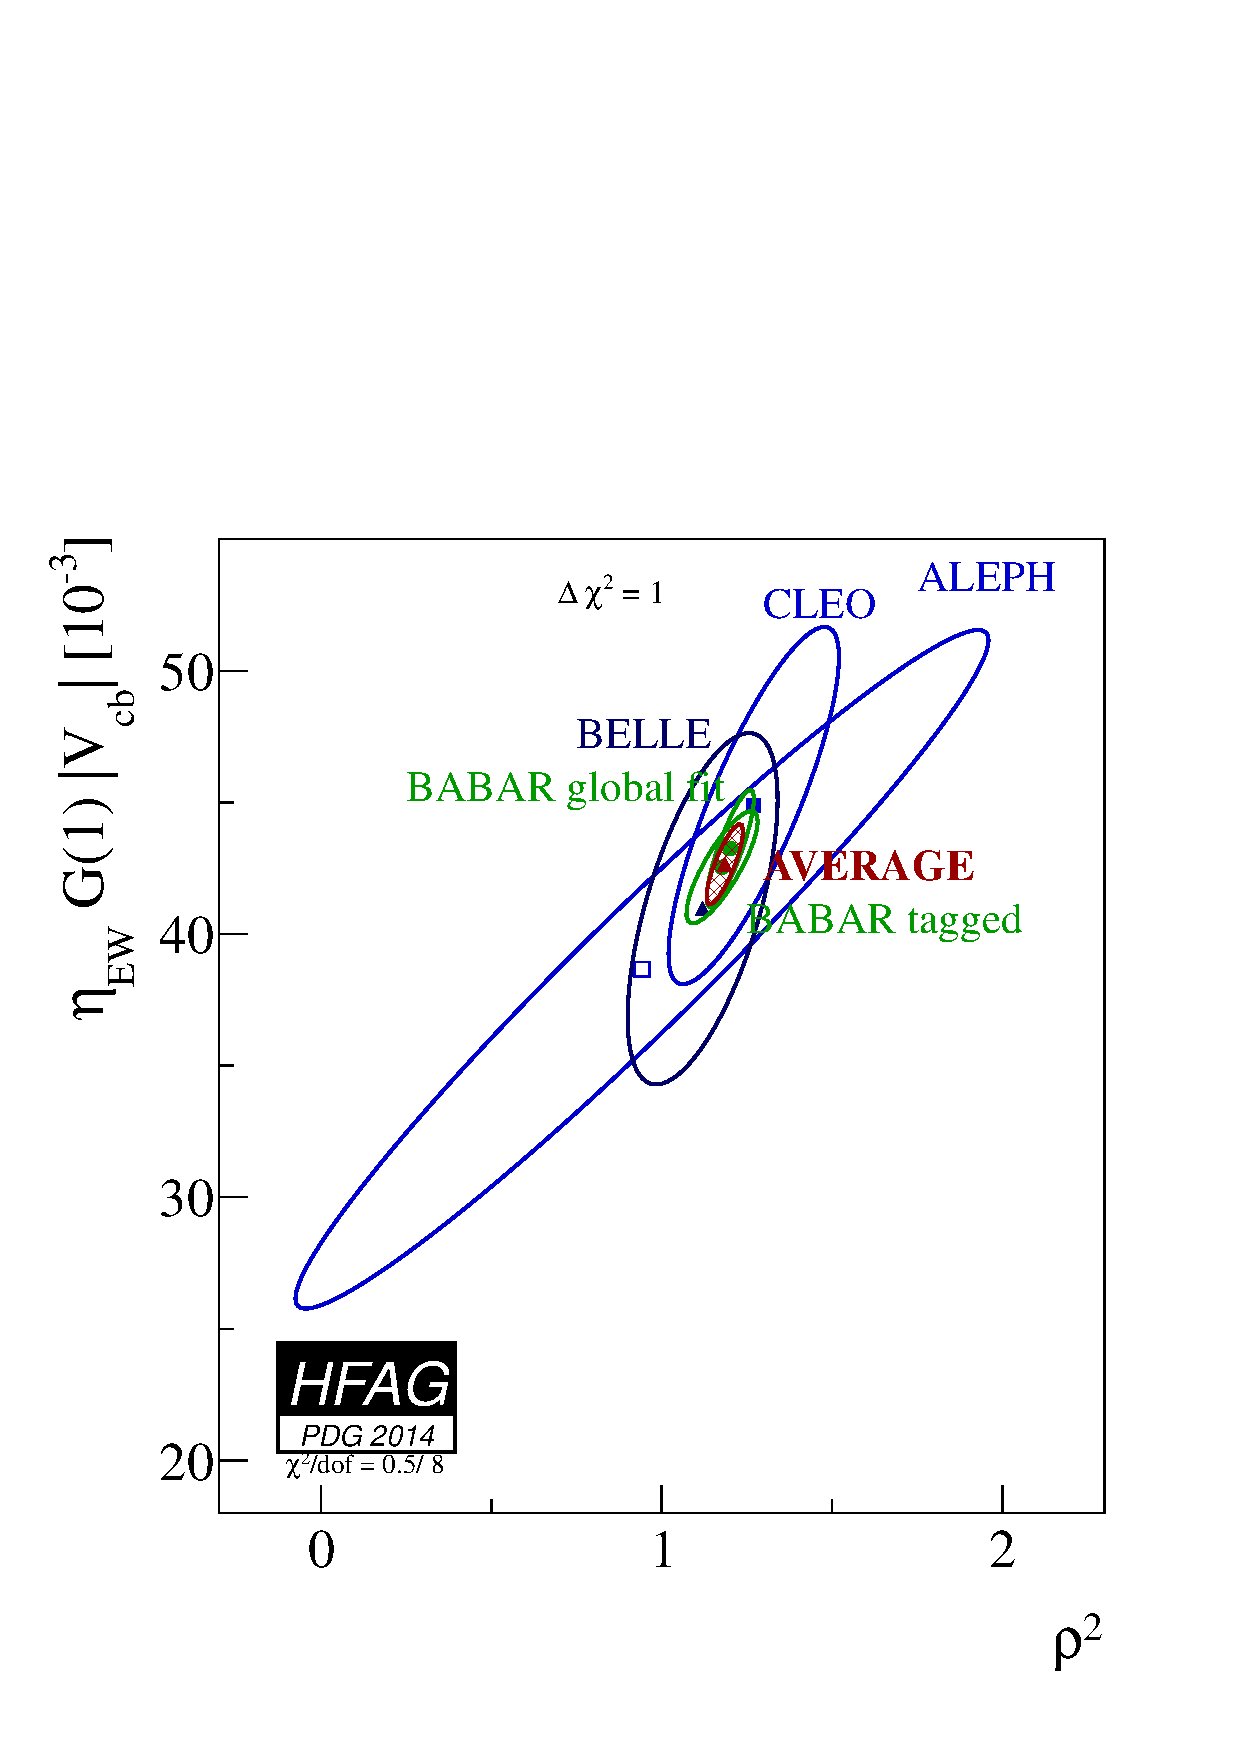
\includegraphics[width=8.0cm]{figures/slb/vcbg1_vs_rho2.pdf}
    }
    \put( -0.5,  0.0){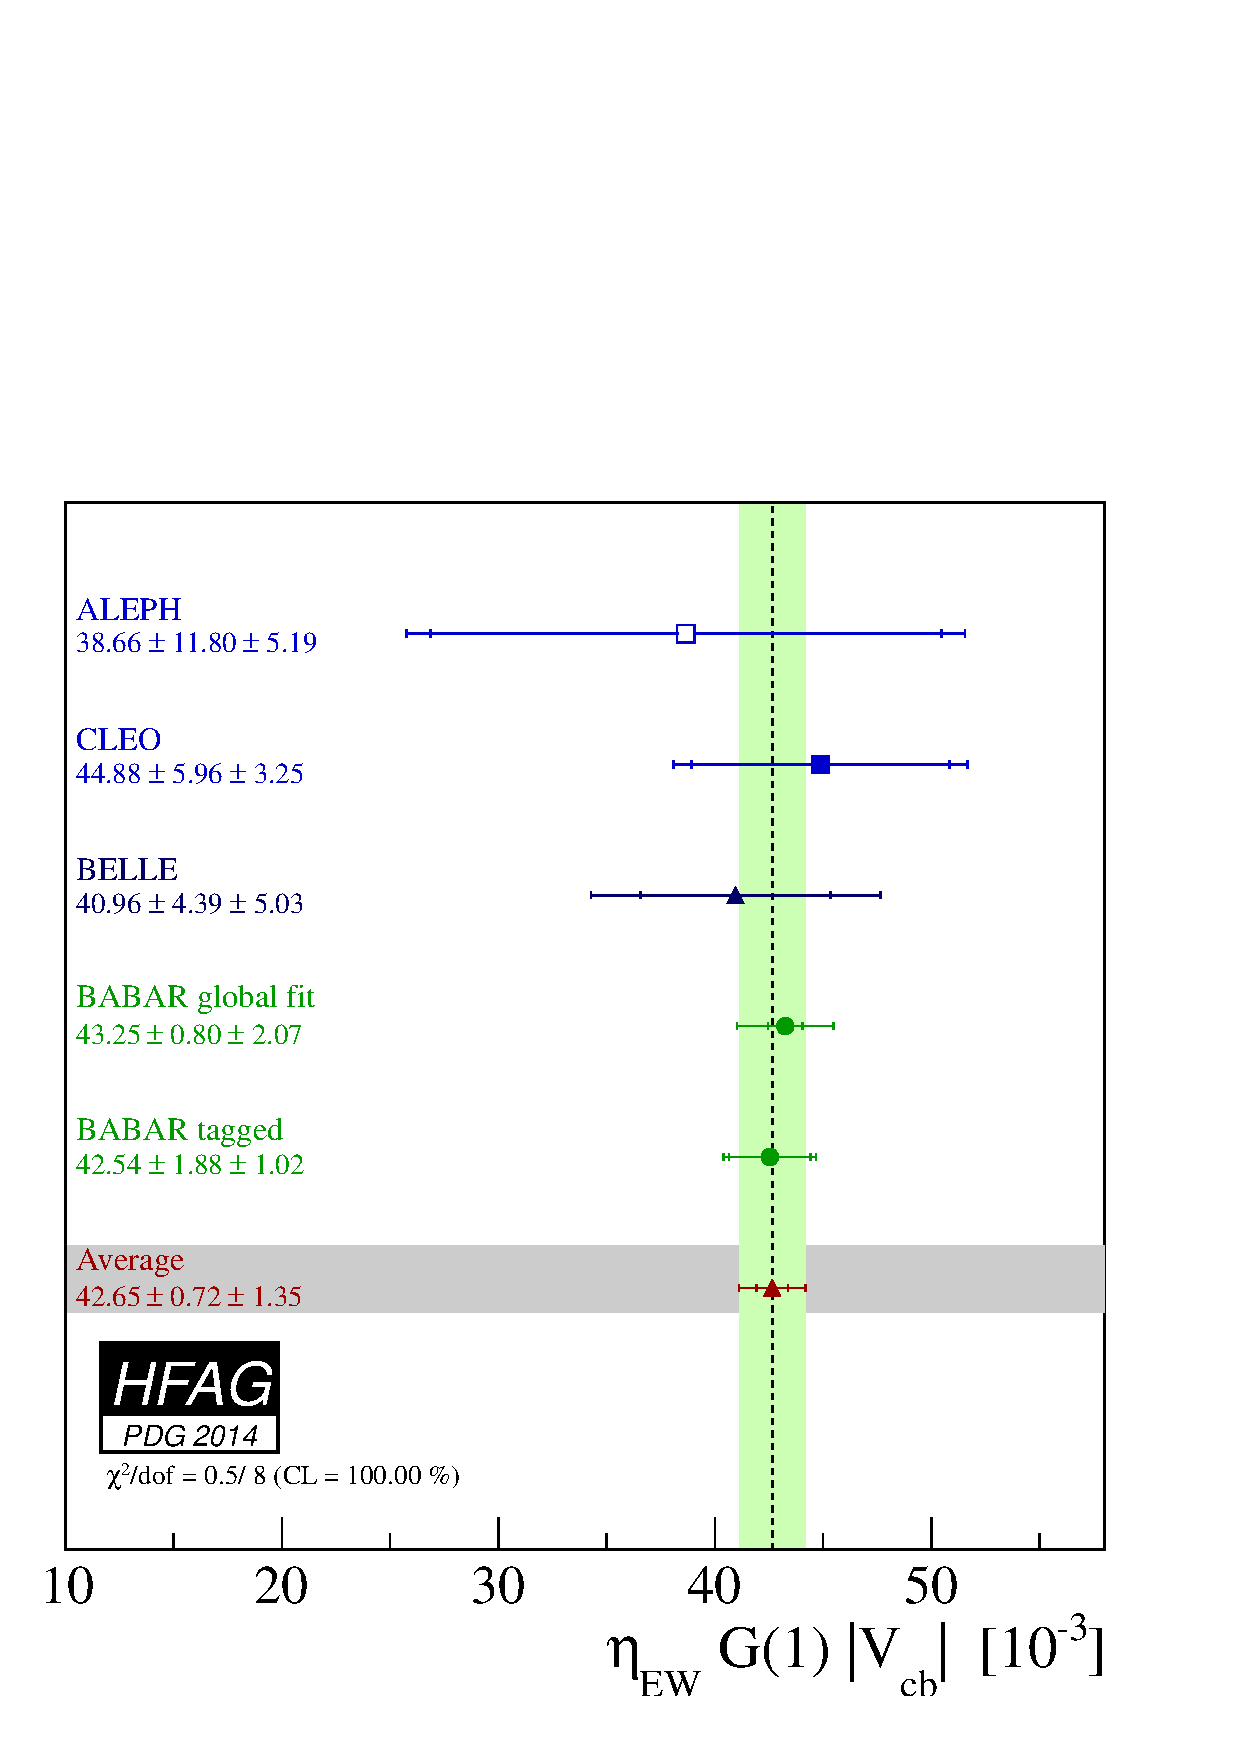
\includegraphics[width=7.5cm]{figures/slb/vcbg1.pdf}
    }
    \put(  5.5,  6.8){{\large\bf a)}}
    \put( 9.4,  6.8){{\large\bf b)}}
  \end{picture}
  \caption{(a) Illustration of the $\eta_\mathrm{EW}{\cal G}(1)\vcb$
    average. (b) Illustration of the $\eta_\mathrm{EW}{\cal G}(1)\vcb$
    vs.\ $\rho^2$ average. The error ellipses correspond  to
    $\Delta\chi^2 = 1$ (CL=39\%).}
  \label{fig:vcbg1}
  \end{center}
\end{figure}

The most recent lattice QCD result obtained for the form factor
normalization $\eta_\mathrm{EW}{\cal G}(1)$ is~\cite{Okamoto:2004xg}
\begin{equation}
  \eta_\mathrm{EW}{\cal G}(1) = 1.081\pm 0.024~,
\end{equation}
which can be used to turn Eq.~\ref{eq:vcbg1} into a determination of
$\vcb$,
\begin{equation}
  \vcb = (39.45\pm 1.42_{\rm exp}\pm 0.88_{\rm th})\times 10^{-3}~,
\end{equation}
where the first error is experimental and the second theoretical. This
number is in excellent agreement with $\vcb$ obtained from decays
$\bar B\to D^*\ell^-\bar\nu_\ell$ (Eq.~\ref{eq:vcbdstar}).

From each rescaled measurement in Table~\ref{tab:vcbg1}, we have
calculated the $\bar B\to D\ell^-\bar\nu_\ell$ form factor ${\cal
  G}(w)$ and, by numerical integration, the branching ratio of the
decay $\BzbDplnu$. The results are quoted in Table~\ref{tab:dlnuIso} and
illustrated in Fig.~\ref{fig:brdlIso}. The branching ratio found for
the average values of $\eta_\mathrm{EW}{\cal G}(1)\vcb$ and $\rho^2$ is
\begin{equation}
  \cbf(\BzbDplnu)=(2.13\pm 0.09)\%~.
\end{equation}
% ----------------------------------------------------------------------0
\begin{table}[!htb]
\caption{$\bar B^0\to D^+\ell^-\bar\nu_\ell$ branching fractions
  calculated from the rescaled measurements in Table~\ref{tab:vcbg1},
  asumming the CLN parameterization of the form factor~\cite{CLN}. The
  fit assumes isospin symmetry.}
\begin{center}
\resizebox{0.99\textwidth}{!}{
\begin{tabular}{|l|c|c|}
  \hline
  Experiment
  & $\cbf(\bar B^0\to D^+\ell^-\bar\nu_\ell)$ [\%] (calculated)
  & $\cbf(\bar B^0\to D^+\ell^-\bar\nu_\ell)$ [\%] (published)\\
  \hline \hline
  ALEPH~\hfill\cite{Buskulic:1996yq}
  & $2.16\pm 0.18_{\rm stat}\pm 0.46_{\rm syst}$
  & $2.35\pm 0.20_{\rm stat}\pm 0.44_{\rm syst}$\\
  CLEO~\hfill\cite{Bartelt:1998dq}
  & $2.19\pm 0.16_{\rm stat}\pm 0.35_{\rm syst}$
  & $2.20\pm 0.16_{\rm stat}\pm 0.19_{\rm syst}$\\
  \belle~\hfill\cite{Abe:2001yf}
  & $2.07\pm 0.12_{\rm stat}\pm 0.52_{\rm syst}$
  & $2.13\pm 0.12_{\rm stat}\pm 0.39_{\rm syst}$\\
  \babar global fit~\hfill\cite{Aubert:2009_1}
  & $2.18\pm 0.03_{\rm stat}\pm 0.13_{\rm syst}$
  & $2.34\pm 0.03_{\rm stat}\pm 0.13_{\rm syst}$\\
  \babar tagged~\hfill\cite{Aubert:2009_2}
  & $2.12\pm 0.10_{\rm stat}\pm 0.06_{\rm syst}$
  & $2.23\pm 0.11_{\rm stat}\pm 0.11_{\rm syst}$\\
  \hline 
  {\bf Average}
  & \mathversion{bold}$2.13\pm 0.03_{\rm stat}\pm 0.09_{\rm syst}$
  & \mathversion{bold}$\chi^2/\dof = 0.5/8$ (CL=$100.0\%$)\\
  \hline 
\end{tabular}
}
\end{center}
\label{tab:dlnuIso}
\end{table}
% ----------------------------------------------------------------------

\begin{figure}[!ht]
  \begin{center}
    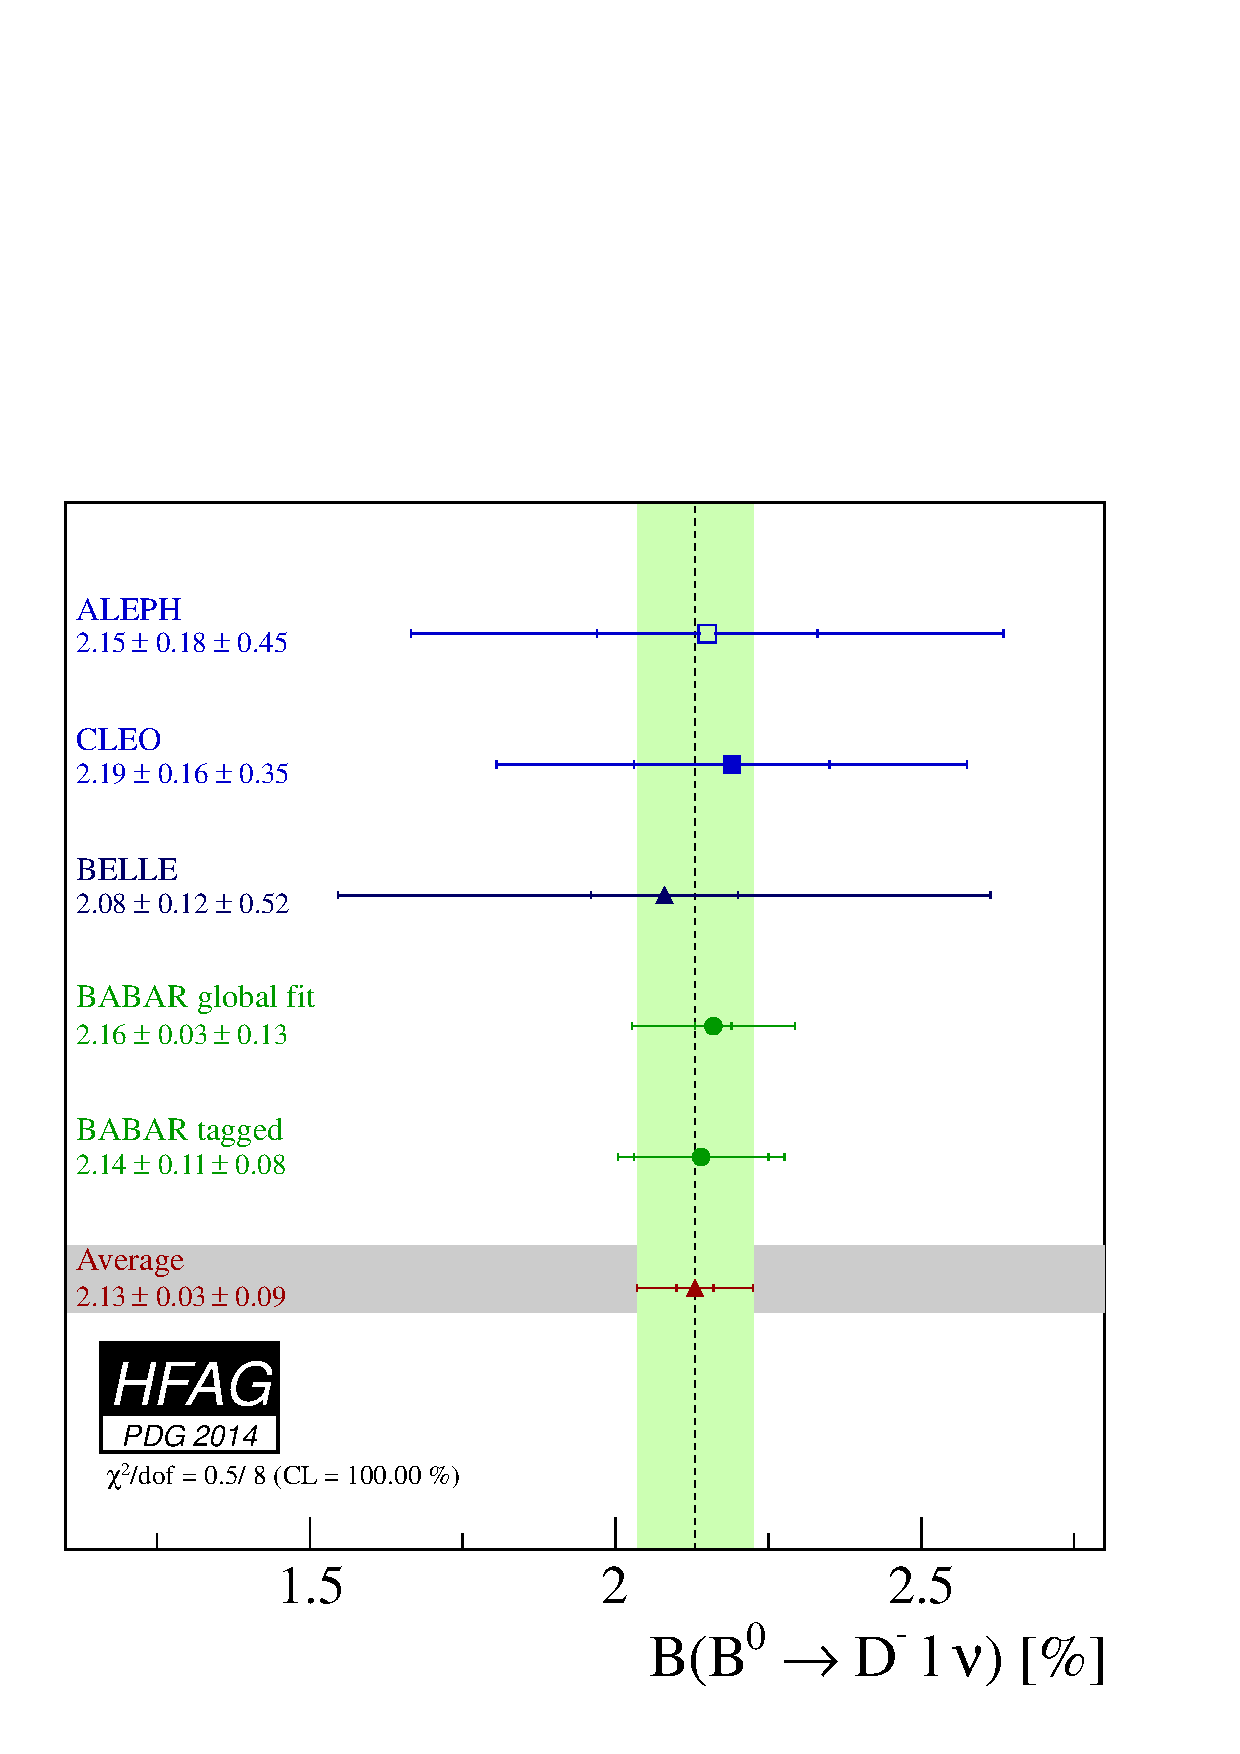
\includegraphics[width=7.55cm]{figures/slb/br_dl_iso.pdf}
    \caption{Illustration of Table~\ref{tab:dlnuIso}.} \label{fig:brdlIso}
  \end{center}
\end{figure}

We have also performed simple 1-dimensional averages of measurements
of $\BzbDplnu$ and $B^-\to D^0\ell^-\bar\nu_\ell$. These fits are
shown Tables~\ref{tab:dlnu} and \ref{tab:d0lnu}.
% ----------------------------------------------------------------------0
\begin{table}[!htb]
\caption{Average of the $\BzbDplnu$ branching fraction
  measurements. This fit uses only measurements of $\BzbDplnu$.}
\begin{center}
\begin{tabular}{|l|c|c|}
  \hline
  Experiment
  & $\cbf(\BzbDplnu)$ [\%] (rescaled)
  & $\cbf(\BzbDplnu)$ [\%] (published)\\
  \hline \hline
  ALEPH~\hfill\cite{Buskulic:1996yq}
  & $2.28\pm 0.18_{\rm stat}\pm 0.35_{\rm syst}$
  & $2.35\pm 0.20_{\rm stat}\pm 0.44_{\rm syst}$\\
  CLEO~\hfill\cite{Bartelt:1998dq}
  & $2.13\pm 0.13_{\rm stat}\pm 0.15_{\rm syst}$
  & $2.20\pm 0.16_{\rm stat}\pm 0.19_{\rm syst}$\\
  \belle~\hfill\cite{Abe:2001yf}
  & $2.11\pm 0.12_{\rm stat}\pm 0.39_{\rm syst}$
  & $2.13\pm 0.12_{\rm stat}\pm 0.39_{\rm syst}$\\
  \babar~\hfill\cite{Aubert:vcbExcl}
  & $2.22\pm 0.11_{\rm stat}\pm 0.12_{\rm syst}$
  & $2.21\pm 0.11_{\rm stat}\pm 0.12_{\rm syst}$\\
  \hline 
  {\bf Average}
  & \mathversion{bold}$2.19\pm 0.06_{\rm stat}\pm 0.10_{\rm syst}$
  & \mathversion{bold}$\chi^2/\dof = 0.2/3$ (CL=$97.3\%$)\\
  \hline 
\end{tabular}
\end{center}
\label{tab:dlnu}
\end{table}
% ----------------------------------------------------------------------

% ----------------------------------------------------------------------0
\begin{table}[!htb]
\caption{Average of the $B^-\to D^0\ell^-\bar\nu_\ell$ branching fraction
  measurements. This fit uses only measurements of $B^-\to
  D^0\ell^-\bar\nu_\ell$.}
\begin{center}
\begin{tabular}{|l|c|c|}
  \hline
  Experiment
  & $\cbf(B^-\to D^0\ell^-\bar\nu_\ell)$ [\%] (rescaled)
  & $\cbf(B^-\to D^0\ell^-\bar\nu_\ell)$ [\%] (published)\\
  \hline \hline
  CLEO~\hfill\cite{Bartelt:1998dq}
  & $2.21\pm 0.13_{\rm stat}\pm 0.17_{\rm syst}$
  & $2.32\pm 0.17_{\rm stat}\pm 0.20_{\rm syst}$\\
  \babar~\hfill\cite{Aubert:vcbExcl}
  & $2.28\pm 0.09_{\rm stat}\pm 0.09_{\rm syst}$
  & $2.33\pm 0.09_{\rm stat}\pm 0.09_{\rm syst}$\\
  \hline
  {\bf Average}
  & \mathversion{bold}$2.26\pm 0.07_{\rm stat}\pm 0.08_{\rm syst}$
  & \mathversion{bold}$\chi^2/\dof = 0.1/1$ (CL=$76.0\%$)\\
  \hline
\end{tabular}
\end{center}
\label{tab:d0lnu}
\end{table}
% ----------------------------------------------------------------------


%===================================================================
% D** 
%===================================================================

\mysubsubsection{$\bar{B} \to D^{(*)}\pi \ell^-\bar{\nu}_{\ell}$}
\label{slbdecays_dpilnu}
% --------------------

The average inclusive branching fractions for $\bar{B} \to D^{*}\pi \ell^-\bar{\nu}_{\ell}$
decays, where no constrain is applied to the hadronic $D^{(*)}\pi$ system, 
are determined by the
combination of the results provided in Table~\ref{tab:dpilnu} for 
$\bar{B}^0 \to D^0 \pi^+ \ell^-\bar{\nu}_{\ell}$, $\bar{B}^0 \to D^{*0} \pi^+
\ell^-\bar{\nu}_{\ell}$, 
$B^- \to D^+ \pi^-
\ell^-\bar{\nu}_{\ell}$, and $B^- \to D^{*+} \pi^- \ell^-\bar{\nu}_{\ell}$.
The measurements included in the average 
are scaled to a consistent set of input
parameters and their errors~\cite{HFAG_sl:inputparams}.
For both the \babar\ and Belle results, the $B$ semileptonic signal yields are
 extracted from a fit to the missing mass squared in a sample of fully
 reconstructed \BB\ events.  
Figure~\ref{fig:brdpil} illustrates the measurements and the
resulting average.

% ----------------------------------------------------------------------
\begin{table}[!htb]
\caption{Average of the branching fraction $B \to D^{(*)} \pi^- \ell^-\bar{\nu}_{\ell}$ and individual
results.}
\begin{center}
\begin{tabular}{|l|c c|}\hline
Experiment                                 &$\cbf(B^- \to D^+ \pi^- \ell^-\bar{\nu}_{\ell}) [\%]$ (rescaled) &\\
\hline
\belle  ~\hfill\cite{Live:Dss}           &$0.42 \pm0.04_{\rm stat} \pm0.05_{\rm syst}$  & \\
\babar  ~\hfill\cite{Aubert:vcbExcl}       &$0.42 \pm0.06_{\rm stat} \pm0.03_{\rm syst}$ & \\
\hline 
{\bf Average}                              &\mathversion{bold}$0.42 \pm0.05$  
   &\mathversion{bold}$\chi^2/\dof = 0.001$ (CL=$97\%$)  \\
\hline\hline

Experiment                                 &$\cbf(B^- \to D^{*+} \pi^- \ell^-\bar{\nu}_{\ell}) [\%]$ (rescaled) & \\
\hline\hline 
\belle  ~\hfill\cite{Live:Dss}           &$0.67 \pm0.08_{\rm stat} \pm0.07_{\rm syst}$  
& \\
\babar  ~\hfill\cite{Aubert:vcbExcl}       &$0.59 \pm0.05_{\rm stat} \pm0.04_{\rm syst}$  
& \\
\hline 
{\bf Average}                              &\mathversion{bold}$0.61 \pm0.05$  
 & \mathversion{bold}$\chi^2/\dof = 0.15$ (CL=$69\%$)    \\
\hline \hline

Experiment                               &$\cbf(\bar{B}^0 \to D^0 \pi^+ \ell^-\bar{\nu}_{\ell}) [\%]$ (rescaled) & \\
\hline\hline 
\belle  ~\hfill\cite{Live:Dss}           &$0.43 \pm0.07_{\rm stat} \pm0.05_{\rm syst}$ &  \\
\babar  ~\hfill\cite{Aubert:vcbExcl}     &$0.43 \pm0.08_{\rm stat} \pm0.03_{\rm syst}$ &  \\
\hline 
{\bf Average}                              &\mathversion{bold}$0.43 \pm0.06$  
   &\mathversion{bold}$\chi^2/\dof = 0.002$ (CL=$97\%$)  \\
\hline\hline

Experiment                                 &$\cbf(\bar{B}^0 \to D^{*0} \pi^+\ell^-\bar{\nu}_{\ell}) [\%]$ (rescaled) & \\
\hline\hline 
\belle  ~\hfill\cite{Live:Dss}           &$0.57 \pm0.21_{\rm stat} \pm0.07_{\rm syst}$  & \\
\babar  ~\hfill\cite{Aubert:vcbExcl}       &$0.48 \pm0.08_{\rm stat} \pm0.04_{\rm syst}$ & \\ 
\hline 
{\bf Average}                              &\mathversion{bold}$0.49 \pm0.08$  
   &\mathversion{bold}$\chi^2/\dof = 0.15$ (CL=$69\%$)  \\
\hline\hline

\end{tabular}
\end{center}
\label{tab:dpilnu}
\end{table}
% ----------------------------------------------------------------------



\begin{figure}[!ht]
 \begin{center}
  \unitlength1.0cm % coordinates in cm
  \begin{picture}(14.,8.0)  %ys(25.,6.0)
   \put( -0.5,  0.0){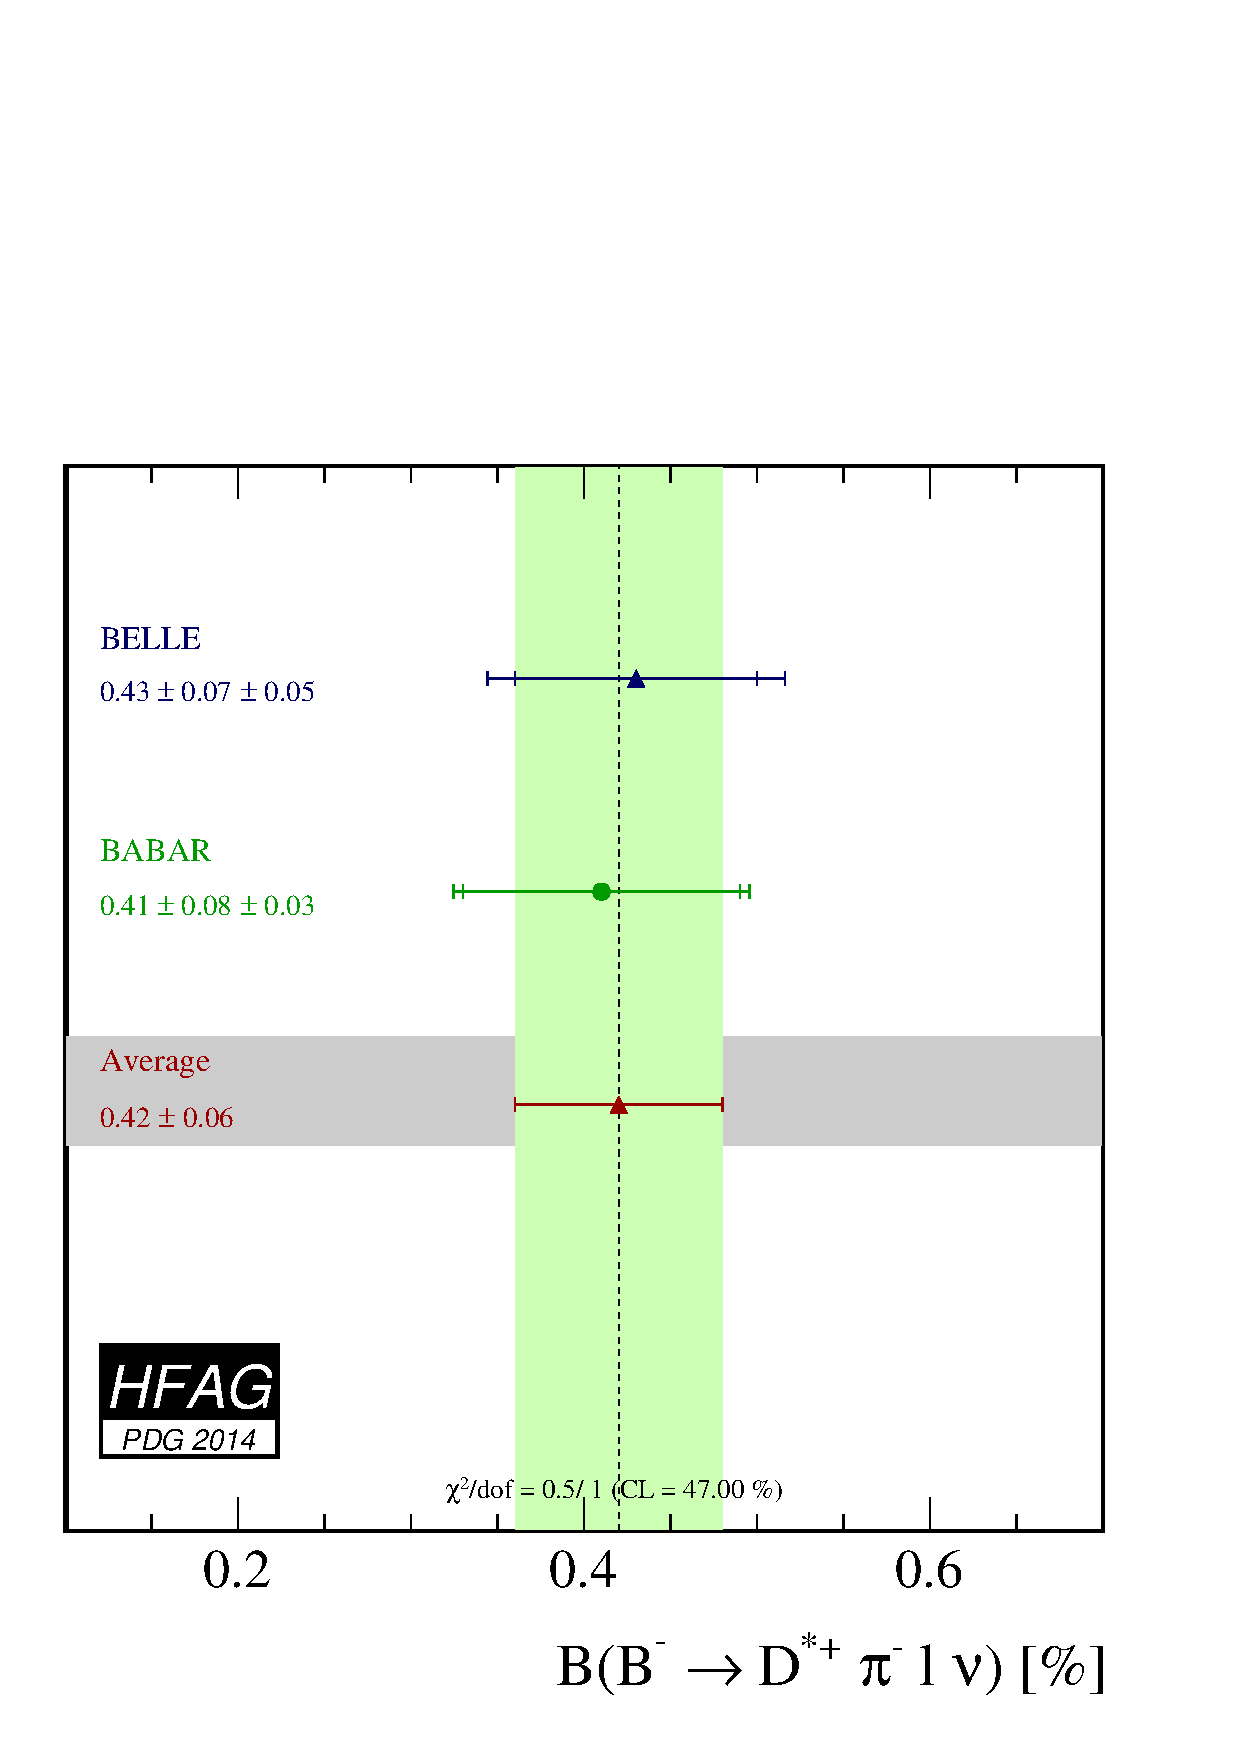
\includegraphics[width=7.55cm]{figures/slb/br_dssIncl-3.pdf}
   }
   \put(  8.0,  0.0){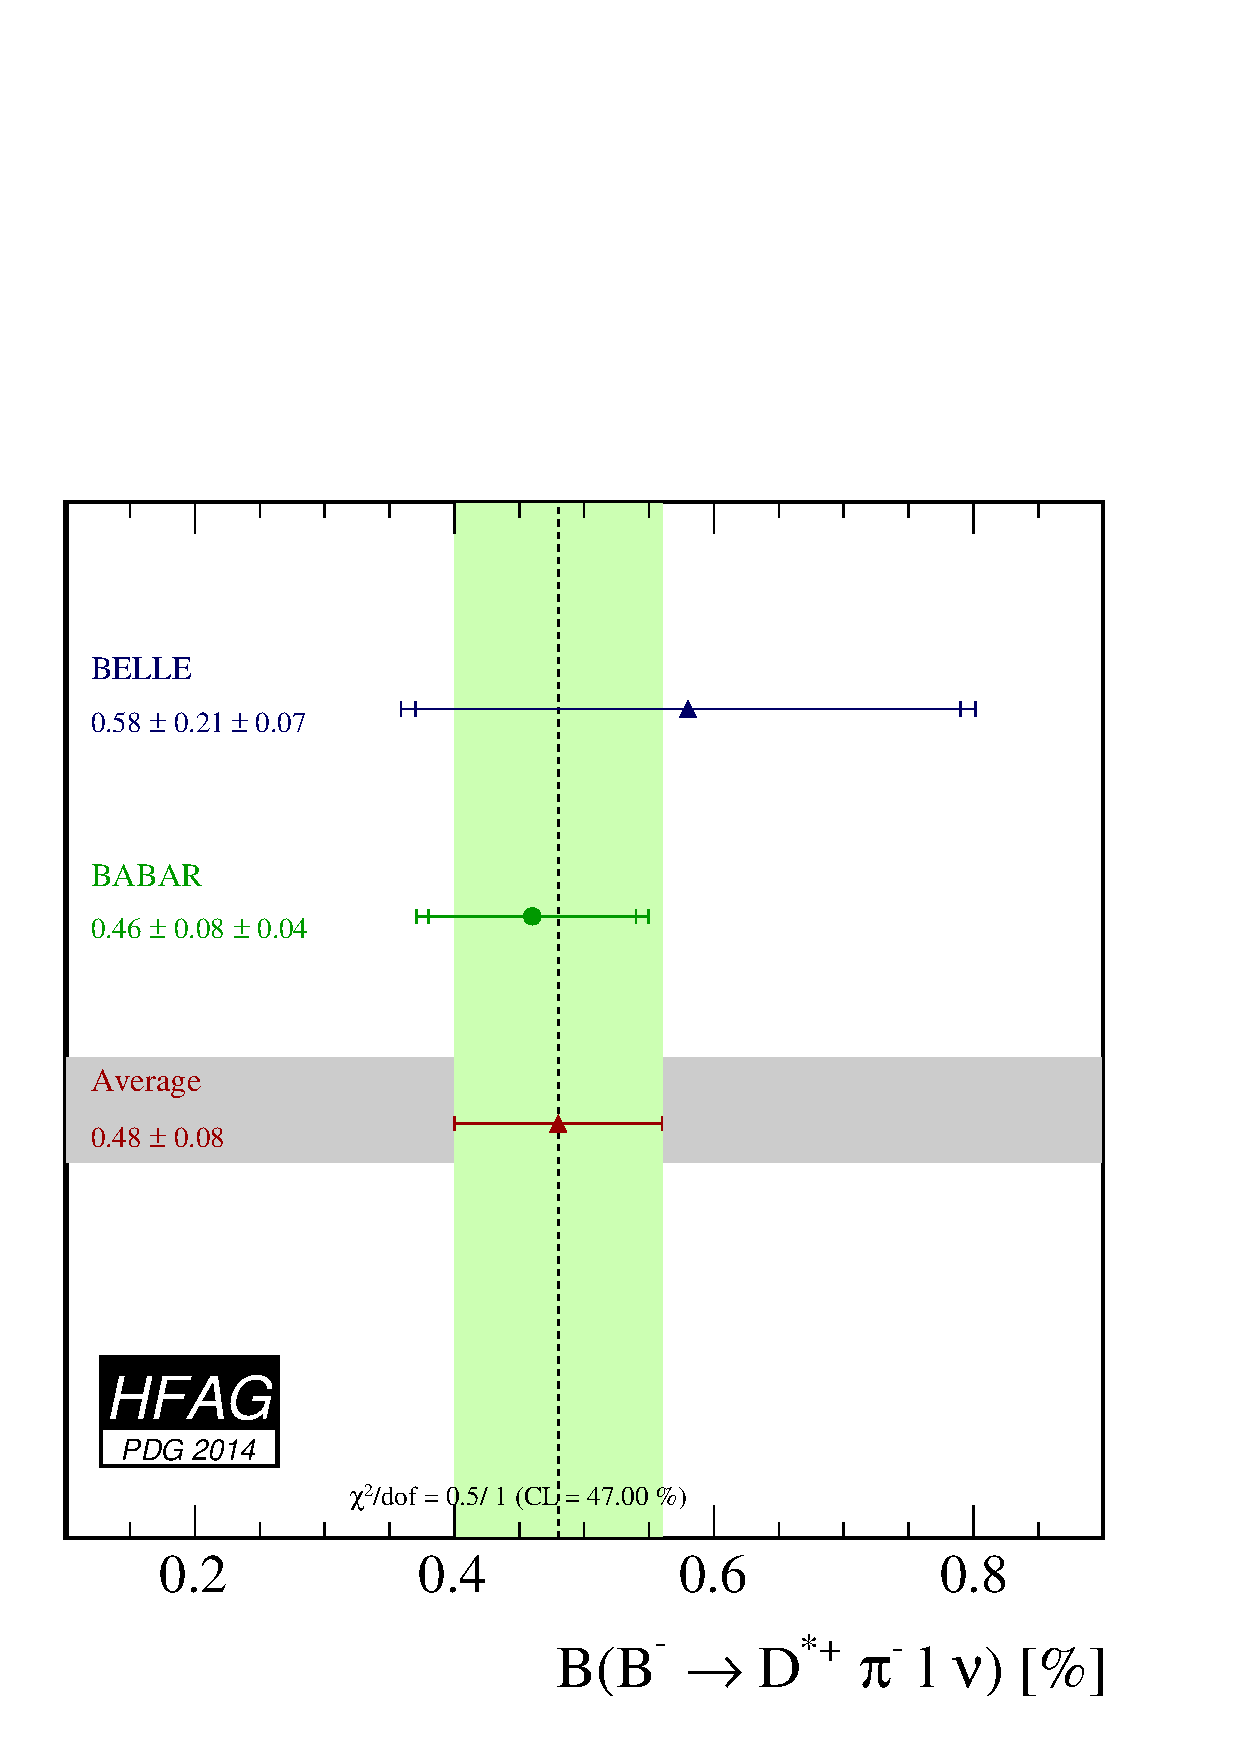
\includegraphics[width=7.8cm]{figures/slb/br_dssIncl-4.pdf}
   }
   \put(  5.5,  6.8){{\large\bf a)}}
   \put( 14.0,  6.8){{\large\bf b)}}
  \end{picture}
  \begin{picture}(14.,8.0)  %ys(25.,6.0)
   \put( -0.5,  0.0){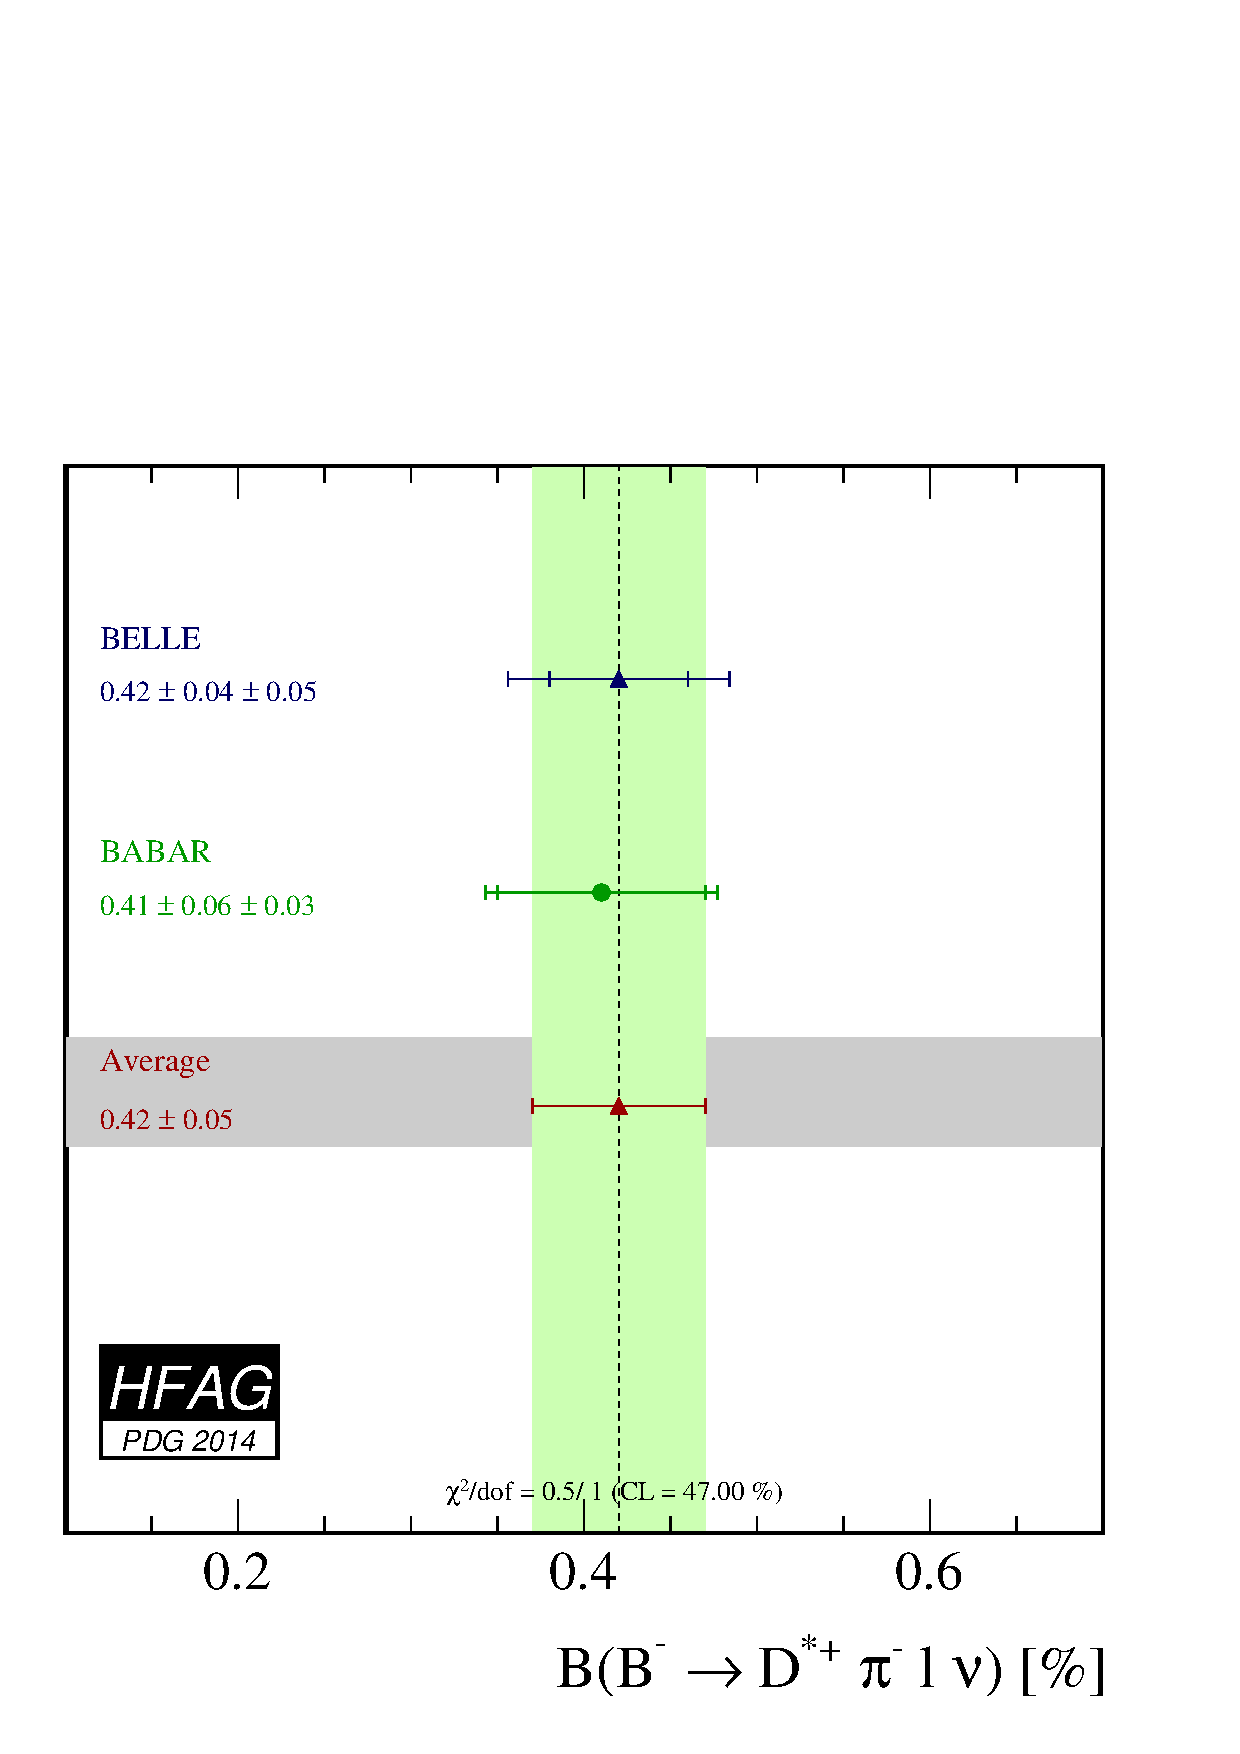
\includegraphics[width=7.55cm]{figures/slb/br_dssIncl-1.pdf}
   }
   \put(  8.0,  0.0){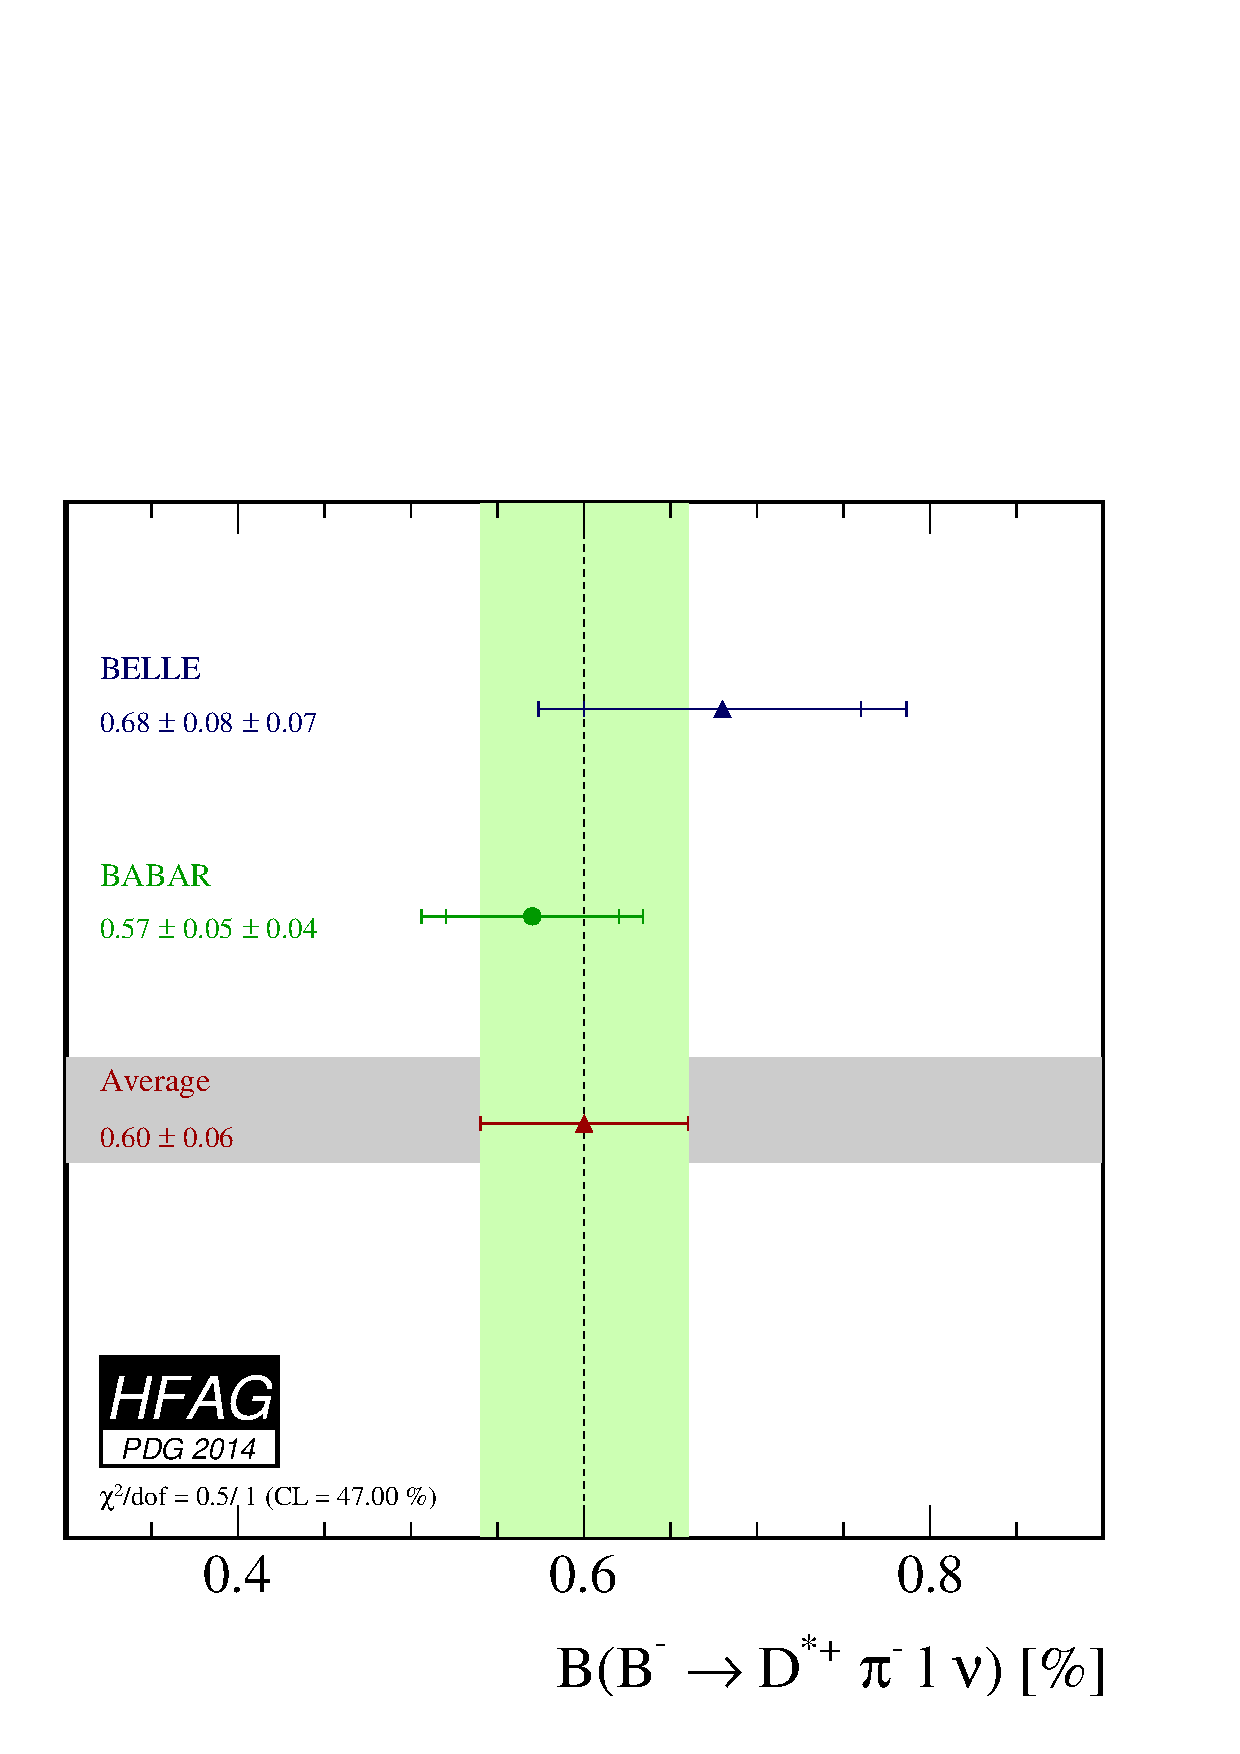
\includegraphics[width=7.8cm]{figures/slb/br_dssIncl-2.pdf}
   }
   \put(  5.5,  6.8){{\large\bf c)}}
   \put( 14.0,  6.8){{\large\bf d)}}
  \end{picture}
  \caption{Average branching fraction  of exclusive semileptonic $B$ decays
(a) $\bar{B}^0 \to D^0 \pi^+ \ell^-\bar{\nu}_{\ell}$, (b) $\bar{B}^0 \to D^{*0} \pi^+
\ell^-\bar{\nu}_{\ell}$, (c) $B^- \to D^+ \pi^-
\ell^-\bar{\nu}_{\ell}$, and (d) $B^- \to D^{*+} \pi^- \ell^-\bar{\nu}_{\ell}$.
The corresponding individual
  results are also shown.}
  \label{fig:brdpil}
 \end{center}
\end{figure}

\mysubsubsection{$\bar{B} \to D^{**} \ell^-\bar{\nu}_{\ell}$}
\label{slbdecays_dsslnu}
% -------------------

The $D^{**}$ mesons contain one charm quark and one light quark with relative angular momentum $L=1$. According to Heavy Quark Symmetry (HQS)~\cite{Isgur:1991wq}, they form one doublet of states with angular momentum $j \equiv s_q + L= 3/2$  $\left[D_1(2420), D_2^*(2460)\right]$ and another doublet with $j=1/2$ $\left[D^*_0(2400), D_1'(2430)\right]$, where $s_q$ is the light quark spin. Parity and angular momentum conservation constrain the decays allowed for each state. The $D_1$ and $D_2^*$ states decay through a D-wave to $D^*\pi$ and $D^{(*)}\pi$, respectively, and have small decay widths, while the $D_0^*$ and $D_1'$  states decay through an S-wave to $D\pi$ and $D^*\pi$ and are very broad.
For the narrow states, the average  are determined by the
combination of the results provided in Table~\ref{tab:dss1lnu} and \ref{tab:dss2lnu} for 
$\cbf(B^- \to D_1^0(D^{*+}\pi^-)\ell^-\bar{\nu}_{\ell})
\times \cbf(D_1^0 \to D^{*+}\pi^-)$ and $\cbf(B^- \to D_2^0(D^{*+}\pi^-)\ell^-\bar{\nu}_{\ell})
\times \cbf(D_2^0 \to D^{*+}\pi^-)$. 
For the broad states, the average are determined by the
combination of the results provided in Table~\ref{tab:dss1plnu} and \ref{tab:dss0lnu} for 
$\cbf(B^- \to D_1'^0(D^{*+}\pi^-)\ell^-\bar{\nu}_{\ell})
\times \cbf(D_1'^0 \to D^{*+}\pi^-)$ and $\cbf(B^- \to D_0^{*0}(D^{+}\pi^-)\ell^-\bar{\nu}_{\ell})
\times \cbf(D_0^{*0} \to D^{+}\pi^-)$. 
The measurements included in the average are scaled to a consistent set of input
parameters and their errors~\cite{HFAG_sl:inputparams}.  

For both the B-factory and the LEP and Tevatron results, the $B$ semileptonic 
signal yields are extracted from a fit to the invariant mass distribution of the $D^{(*)+}\pi^-$ system.
 Apart for the CLEO, \belle and \babar results, the other measurements 
 are for the $\bar{B} \to D^{**}(D^*\pi^-)X \ell^- \bar{\nu}_{\ell}$ final state and 
 we assume that no particles are left in the X system. The \babar tagged measurement \cite{Aubert:2009_4} measures 
 $\bar{B} \to D_2^*(D\pi)X \ell^- \bar{\nu}_{\ell}$ and it has been translated in 
 a result on  $D_2^*\to D^*\pi$ decay mode, assuming 
 ${\cal B}(D_2^*\to D\pi)/{\cal B}(D_2^*\to D^*\pi)=1.54\pm 0.15$ \cite{PDG_2014}. 
Figure~\ref{fig:brdssl} and ~\ref{fig:brdssl2} illustrate the measurements and the
resulting average.

% ----------------------------------------------------------------------0
\begin{table}[!htb]
\caption{Average of the branching fraction $\cbf(B^- \to D_1^0\ell^-\bar{\nu}_{\ell})
\times \cbf(D_1^0 \to D^{*+}\pi^-)$ and individual results. The ALEPH, OPAL and D0 measurements are for the 
$D_1(D^*\pi)X$ final state and we assum that no particles are left in the X system.}
\begin{center}
\resizebox{0.99\textwidth}{!}{
\begin{tabular}{|l|c|c|}\hline
Experiment                                 &$\cbf(B^- \to D_1^0(D^{*+}\pi^-)\ell^-\bar{\nu}_{\ell})
 [\%]$  &$\cbf(B^- \to D_1^0(D^{*+}\pi^-)\ell^-\bar{\nu}_{\ell})
 [\%]$  \\
                                                & (rescaled) & (published) \\

\hline\hline 
ALEPH ~\cite{Aleph:Dss}        &$0.440 \pm0.098_{\rm stat} \pm0.068_{\rm syst}$ 
 &$0.47 \pm0.10_{\rm stat} \pm0.07_{\rm syst}$ \\
OPAL  ~\cite{opal:Dss}         &$0.578 \pm0.210_{\rm stat} \pm0.101_{\rm syst}$  
&$0.70 \pm0.21_{\rm stat} \pm0.10_{\rm syst}$ \\
CLEO  ~\cite{cleo:Dss}         &$0.354 \pm0.085_{\rm stat} \pm0.056_{\rm syst}$ 
 &$0.373 \pm0.085_{\rm stat} \pm0.057_{\rm syst}$ \\
D0  ~\cite{D0:Dss}         &$0.215 \pm0.018_{\rm stat} \pm0.035_{\rm syst}$  
&$0.219 \pm0.018_{\rm stat} \pm0.035_{\rm syst}$ \\
\belle Tagged $B^-$ ~\cite{Live:Dss}           &$0.443 \pm0.070_{\rm stat} \pm0.059_{\rm syst}$  
&$0.42 \pm0.07_{\rm stat} \pm0.07_{\rm syst}$ \\
\belle Tagged $B^0$ ~\cite{Live:Dss}           &$0.612 \pm0.200_{\rm stat} \pm0.077_{\rm syst}$  
&$0.42 \pm0.07_{\rm stat} \pm0.07_{\rm syst}$ \\ 
\babar Tagged ~\cite{Aubert:2009_4}           &$0.278 \pm0.030_{\rm stat} \pm0.028_{\rm syst}$
&$0.29 \pm0.03_{\rm stat} \pm0.03_{\rm syst}$ \\
\babar Untagged $B^-$ ~\cite{Aubert:2008zc}           &$0.295 \pm0.017_{\rm stat} \pm0.016_{\rm syst}$
&$0.30 \pm0.02_{\rm stat} \pm0.02_{\rm syst}$ \\
\babar Untagged $B^0$ ~\cite{Aubert:2008zc}           &$0.299 \pm0.026_{\rm stat} \pm0.027_{\rm syst}$
&$0.30 \pm0.02_{\rm stat} \pm0.02_{\rm syst}$ \\
\hline
{\bf Average}                              &\mathversion{bold}$0.285 \pm0.011 \pm 0.014$ 
    &\mathversion{bold}$\chi^2/\dof = 13.0/8$ (CL=$11.1\%$)  \\
\hline 
\end{tabular}
}
\end{center}
\label{tab:dss1lnu}
\end{table}
% ----------------------------------------------------------------------


% ----------------------------------------------------------------------0
\begin{table}[!htb]
\caption{Average of the branching fraction $\cbf(B^- \to D_2^0(D^{*+}\pi^-)\ell^-\bar{\nu}_{\ell})
\times \cbf(D_2^0 \to D^{*+}\pi^-))$ and individual results. The D0 measurement is for the $D_2^*(D^*\pi)X$
final state and we assume that no particles are left in the X system.
The \babar tagged measurement
has been translated in a result on $D_2^*\to D^*\pi$ decay mode, assuming 
${\cal B}(D_2^*\to D\pi)/{\cal B}(D_2^*\to D^*\pi)=1.54\pm 0.15$, \cite{PDG_2014}.}
\begin{center}
\resizebox{0.99\textwidth}{!}{
\begin{tabular}{|l|c|c|}\hline
Experiment                                 &$\cbf(B^- \to D_2^0(D^{*+}\pi^-)\ell^-\bar{\nu}_{\ell})
) [\%]$  &$\cbf(B^- \to D_2^0(D^{*+}\pi^-)\ell^-\bar{\nu}_{\ell})
) [\%]$  \\
                                                & (rescaled) & (published) \\
\hline\hline 
CLEO  ~\cite{cleo:Dss}         &$0.056 \pm0.066_{\rm stat} \pm0.011_{\rm syst}$ 
 &$0.059 \pm0.066_{\rm stat} \pm0.011_{\rm syst}$ \\
D0  ~\cite{D0:Dss}         &$0.087 \pm0.018_{\rm stat} \pm0.020_{\rm syst}$  
&$0.088 \pm0.018_{\rm stat} \pm0.020_{\rm syst}$ \\
\belle  ~\cite{Live:Dss}           &$0.190 \pm0.060_{\rm stat} \pm0.025_{\rm syst}$  
&$0.18 \pm0.06_{\rm stat} \pm0.03_{\rm syst}$ \\
\babar tagged ~\cite{Aubert:2009_4}           &$0.076 \pm0.013_{\rm stat} \pm0.009_{\rm syst}$
&$0.078 \pm0.013_{\rm stat} \pm0.010_{\rm syst}$ \\
\babar untagged $B^-$ ~\cite{Aubert:2009_5}           &$0.090 \pm0.009_{\rm stat} \pm0.007_{\rm syst}$
&$0.087 \pm0.013_{\rm stat} \pm0.007_{\rm syst}$ \\
\babar untagged $B^0$ ~\cite{Aubert:2009_5}           &$0.067 \pm0.010_{\rm stat} \pm0.004_{\rm syst}$
&$0.087 \pm0.013_{\rm stat} \pm0.007_{\rm syst}$ \\
\hline
{\bf Average}                              &\mathversion{bold}$0.078 \pm0.007 \pm 0.004$ 
    &\mathversion{bold}$\chi^2/\dof = 5.6/5$ (CL=$34.7\%$)  \\
\hline 
\end{tabular}
}
\end{center}
\label{tab:dss2lnu}
\end{table}
% ----------------------------------------------------------------------


% ----------------------------------------------------------------------
\begin{table}[!htb]
\caption{Average of the branching fraction $\cbf(B^- \to D_1^{'0}(D^{*+}\pi^-)\ell^-\bar{\nu}_{\ell})
\times \cbf(D_1^{'0} \to D^{*+}\pi^-))$ and individual results. The DELPHI measurement 
is for the final state $D_1'(D^*\pi)X$ and we assume that no particles are left in the X system.}
\begin{center}
\begin{tabular}{|l|c|c|}\hline
Experiment                                 &$\cbf(B^- \to D_1^{'0}(D^{*+}\pi^-)\ell^-\bar{\nu}_{\ell})
) [\%]$  &$\cbf(B^- \to D_1^{'0}(D^{*+}\pi^-)\ell^-\bar{\nu}_{\ell})
) [\%]$  \\
                                                & (rescaled) & (published) \\
\hline\hline 
DELPHI ~\cite{Abdallah:2005cx}        &$0.74 \pm0.17_{\rm stat} \pm0.18_{\rm syst}$ 
 &$0.83 \pm0.17_{\rm stat} \pm0.18_{\rm syst}$ \\
\belle  ~\cite{Live:Dss}           &$-0.03 \pm0.06_{\rm stat} \pm0.07_{\rm syst}$  
&$-0.03 \pm0.06_{\rm stat} \pm0.07_{\rm syst}$ \\
\babar  ~\cite{Aubert:2009_4}           &$0.26 \pm0.04_{\rm stat} \pm0.04_{\rm syst}$
&$0.27 \pm0.04_{\rm stat} \pm0.05_{\rm syst}$ \\
\hline
{\bf Average}                              &\mathversion{bold}$0.13 \pm 0.03 \pm0.02$ 
    &\mathversion{bold}$\chi^2/\dof = 18./2$ (CL=$0.0001\%$)  \\
\hline 
\end{tabular}
\end{center}
\label{tab:dss1plnu}
\end{table}
% ----------------------------------------------------------------------


% ----------------------------------------------------------------------0
\begin{table}[!htb]
\caption{Average of the branching fraction $\cbf(B^- \to D_0^{*0}(D^{+}\pi^-)\ell^-\bar{\nu}_{\ell})
\times \cbf(D_0^{*0} \to D^{+}\pi^-))$ and individual
results. }
\begin{center}
\begin{tabular}{|l|c|c|}\hline
Experiment                                 &$\cbf(B^- \to D_0^{*0}(D^{+}\pi^-)\ell^-\bar{\nu}_{\ell})
) [\%]$  &$\cbf(B^- \to D_0^{*0}(D^{+}\pi^-)\ell^-\bar{\nu}_{\ell})
) [\%]$ \\
						& (rescaled) & (published) \\
\hline\hline 
\belle Tagged $B^-$ ~\hfill\cite{Live:Dss}           &$0.25 \pm0.04_{\rm stat} \pm0.06_{\rm syst}$  
&$0.24 \pm0.04_{\rm stat} \pm0.06_{\rm syst}$ \\
\belle Tagged $B^0$ ~\hfill\cite{Live:Dss}           &$0.23 \pm0.08_{\rm stat} \pm0.06_{\rm syst}$  
&$0.24 \pm0.04_{\rm stat} \pm0.06_{\rm syst}$ \\
\babar Tagged ~\hfill\cite{Aubert:2009_4}            &$0.31 \pm0.04_{\rm stat} \pm0.05_{\rm syst}$
&$0.26 \pm0.05_{\rm stat} \pm0.04_{\rm syst}$ \\
\hline
{\bf Average}                              &\mathversion{bold}$0.29 \pm 0.03 \pm0.04$ 
    &\mathversion{bold}$\chi^2/\dof = 0.61/2$ (CL=$73.6\%$)  \\
\hline 
\end{tabular}
\end{center}
\label{tab:dss0lnu}
\end{table}
% ----------------------------------------------------------------------



\begin{figure}[!ht]
 \begin{center}
  \unitlength1.0cm % coordinates in cm
  \begin{picture}(14.,8.0)  %ys(25.,6.0)
   \put( -0.5,  0.0){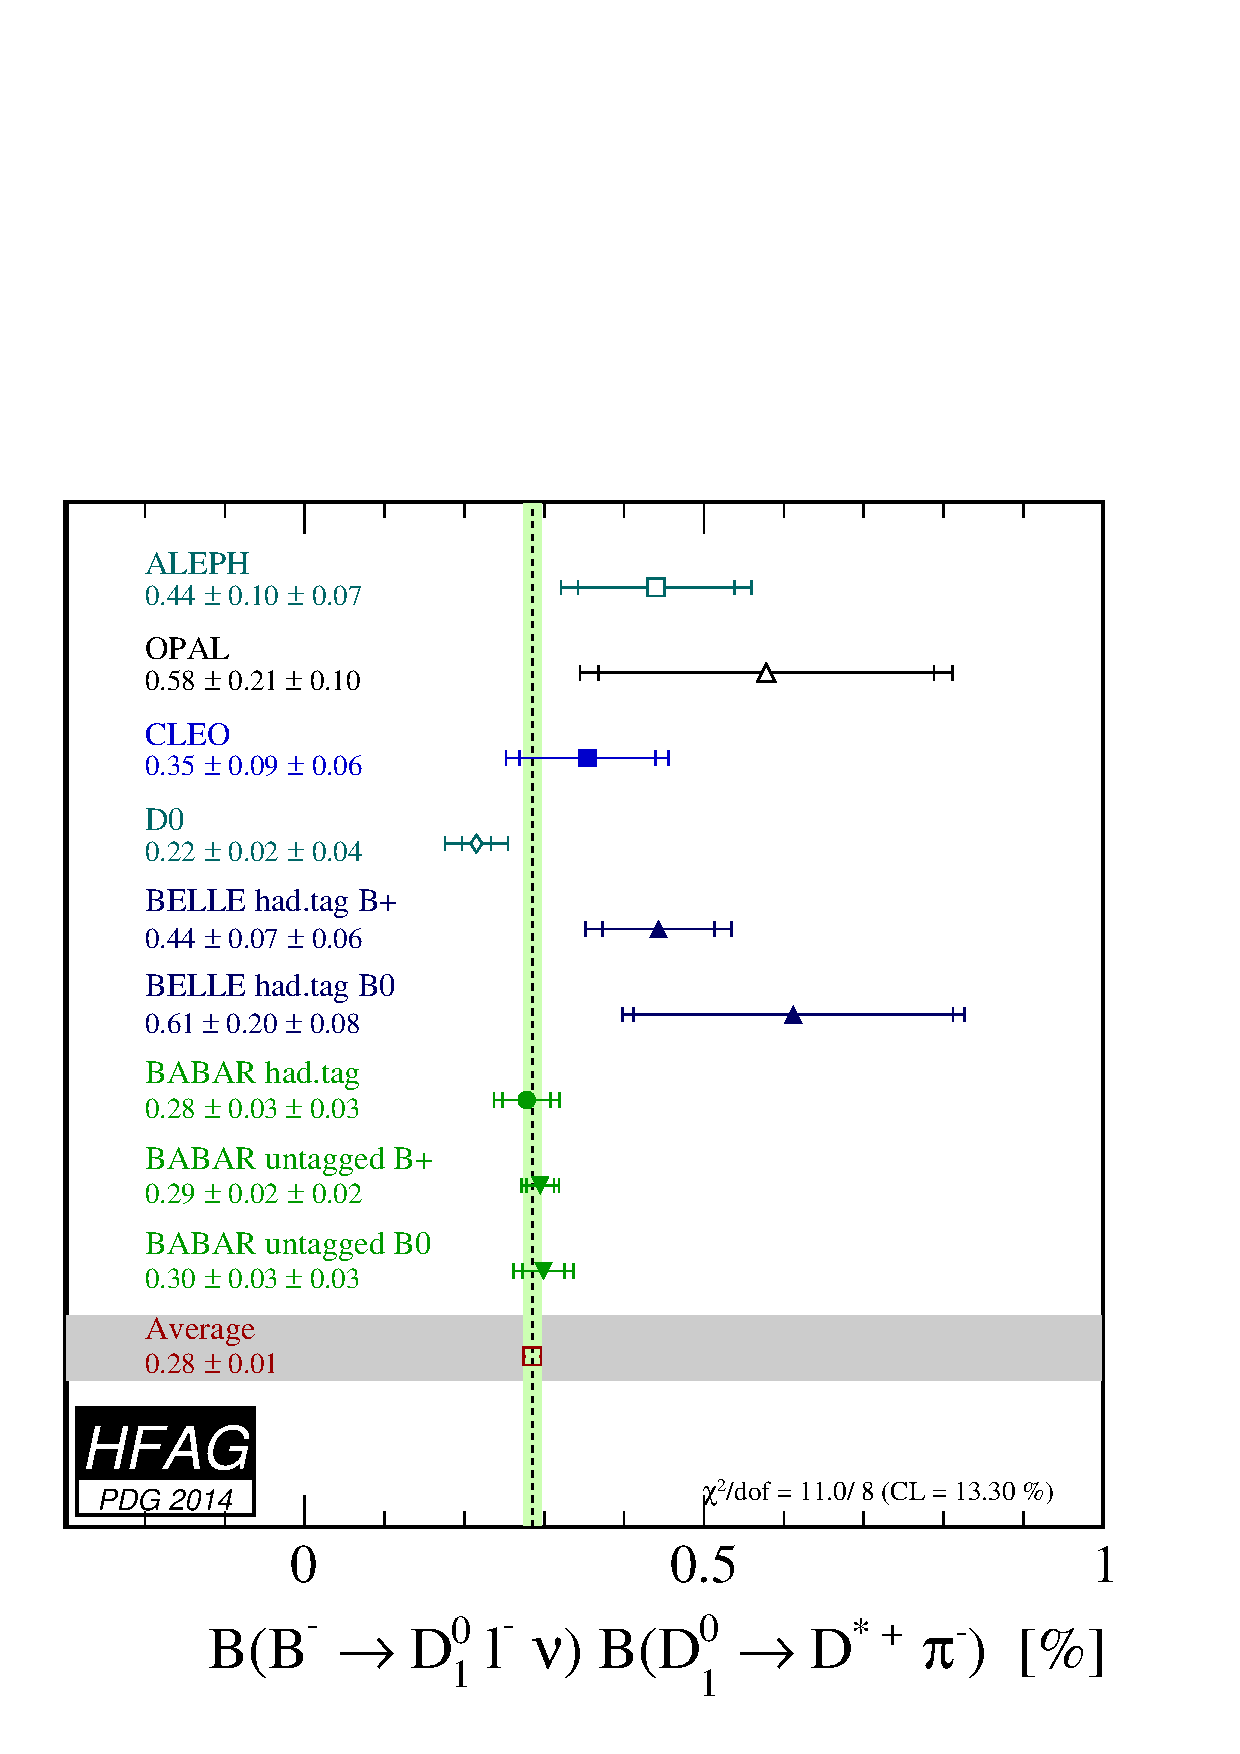
\includegraphics[width=7.8cm]{figures/slb/br_dss1l.pdf}
   }
   \put(  8.0,  0.0){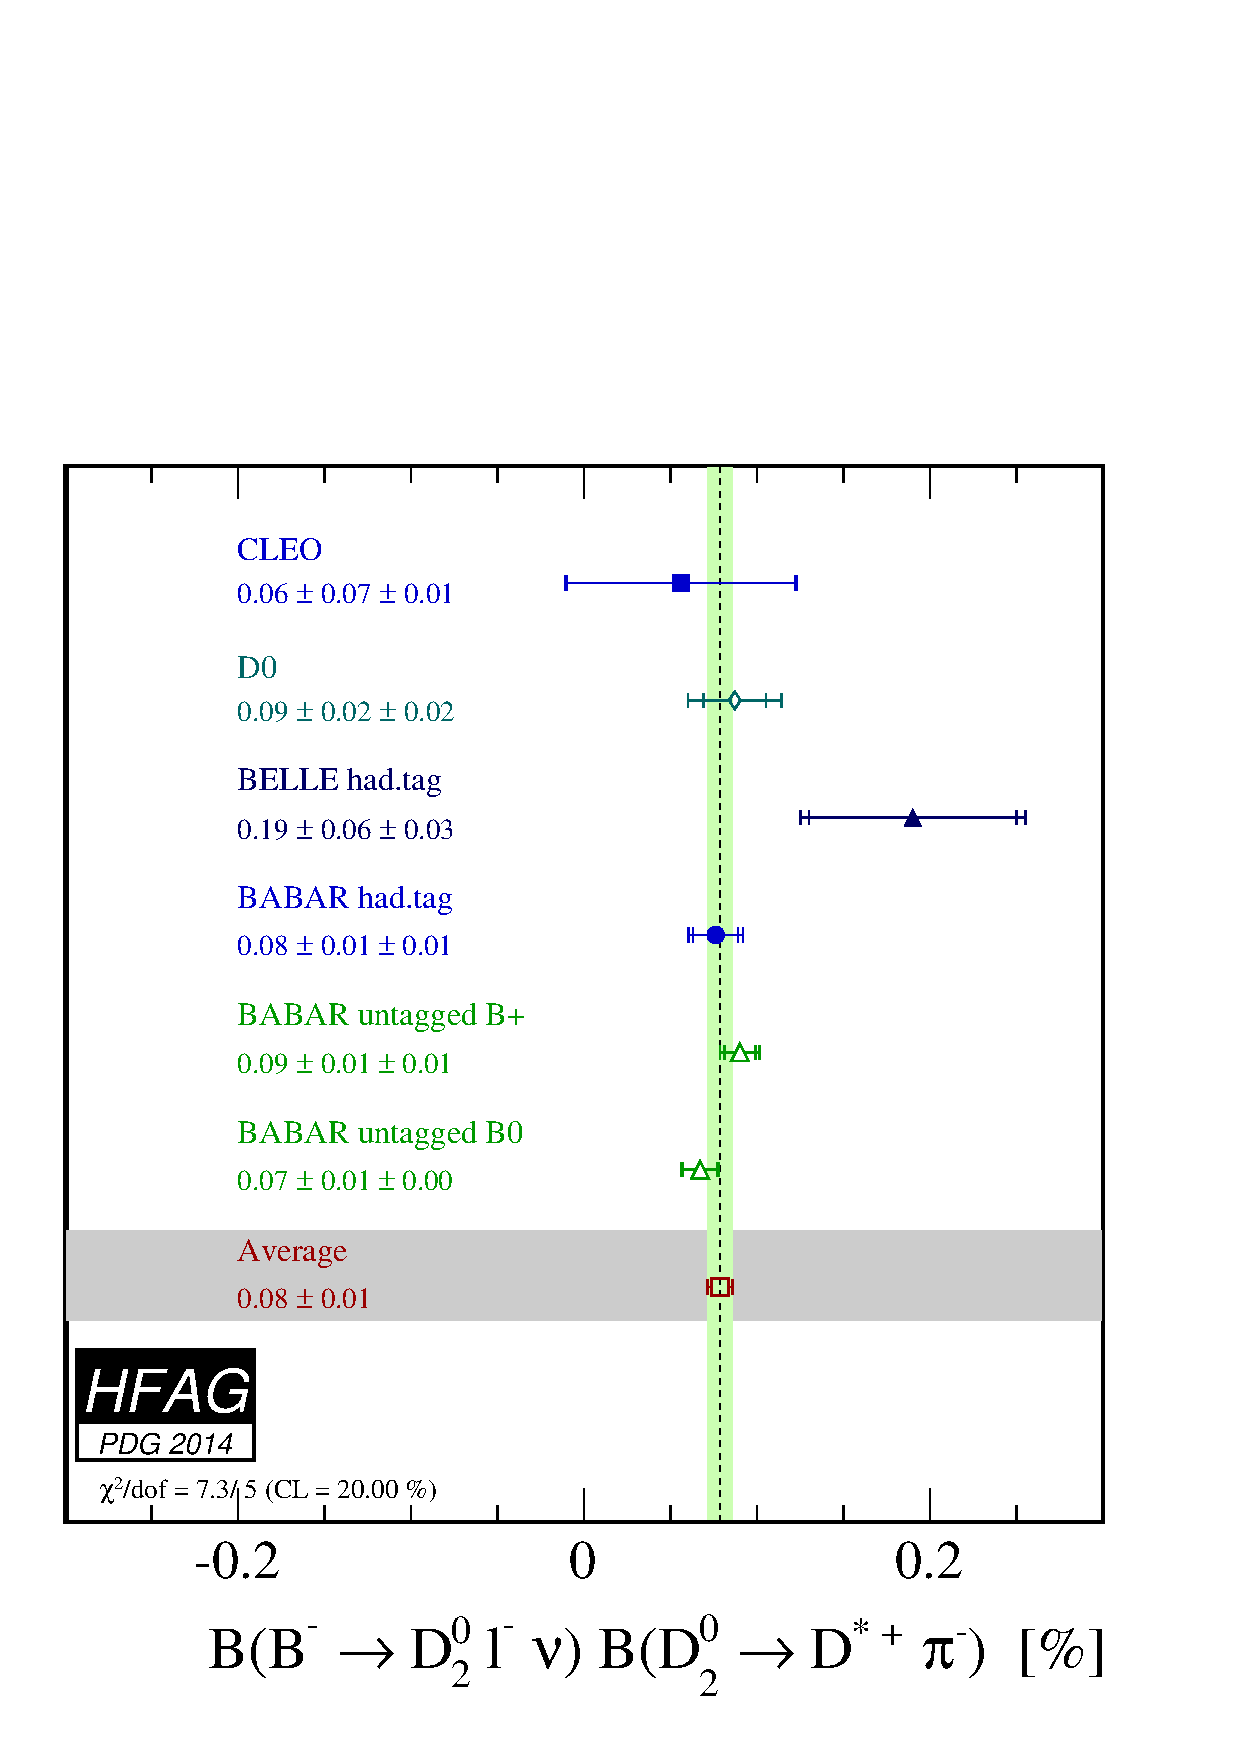
\includegraphics[width=7.55cm]{figures/slb/br_dss2l.pdf}
   }
   \put(  5.5,  7.0){{\large\bf a)}}
   \put( 14.0,  7.0){{\large\bf b)}}
  \end{picture}
  \caption{Average of the product of branching fraction (a) 
  $\cbf(B^- \to D_1^0(D^{*+}\pi^-)\ell^-\bar{\nu}_{\ell})
\times \cbf(D_1^0 \to D^{*+}\pi^-)$ and (b) $\cbf(B^- \to D_2^0(D^{*+}\pi^-)\ell^-\bar{\nu}_{\ell})
\times \cbf(D_2^0 \to D^{*+}\pi^-)$. The corresponding individual results are also shown.}
  \label{fig:brdssl}
 \end{center}
\end{figure}

\begin{figure}[!ht]
 \begin{center}
  \unitlength1.0cm % coordinates in cm
  \begin{picture}(14.,8.0)  %ys(25.,6.0)
   \put( -0.5,  0.0){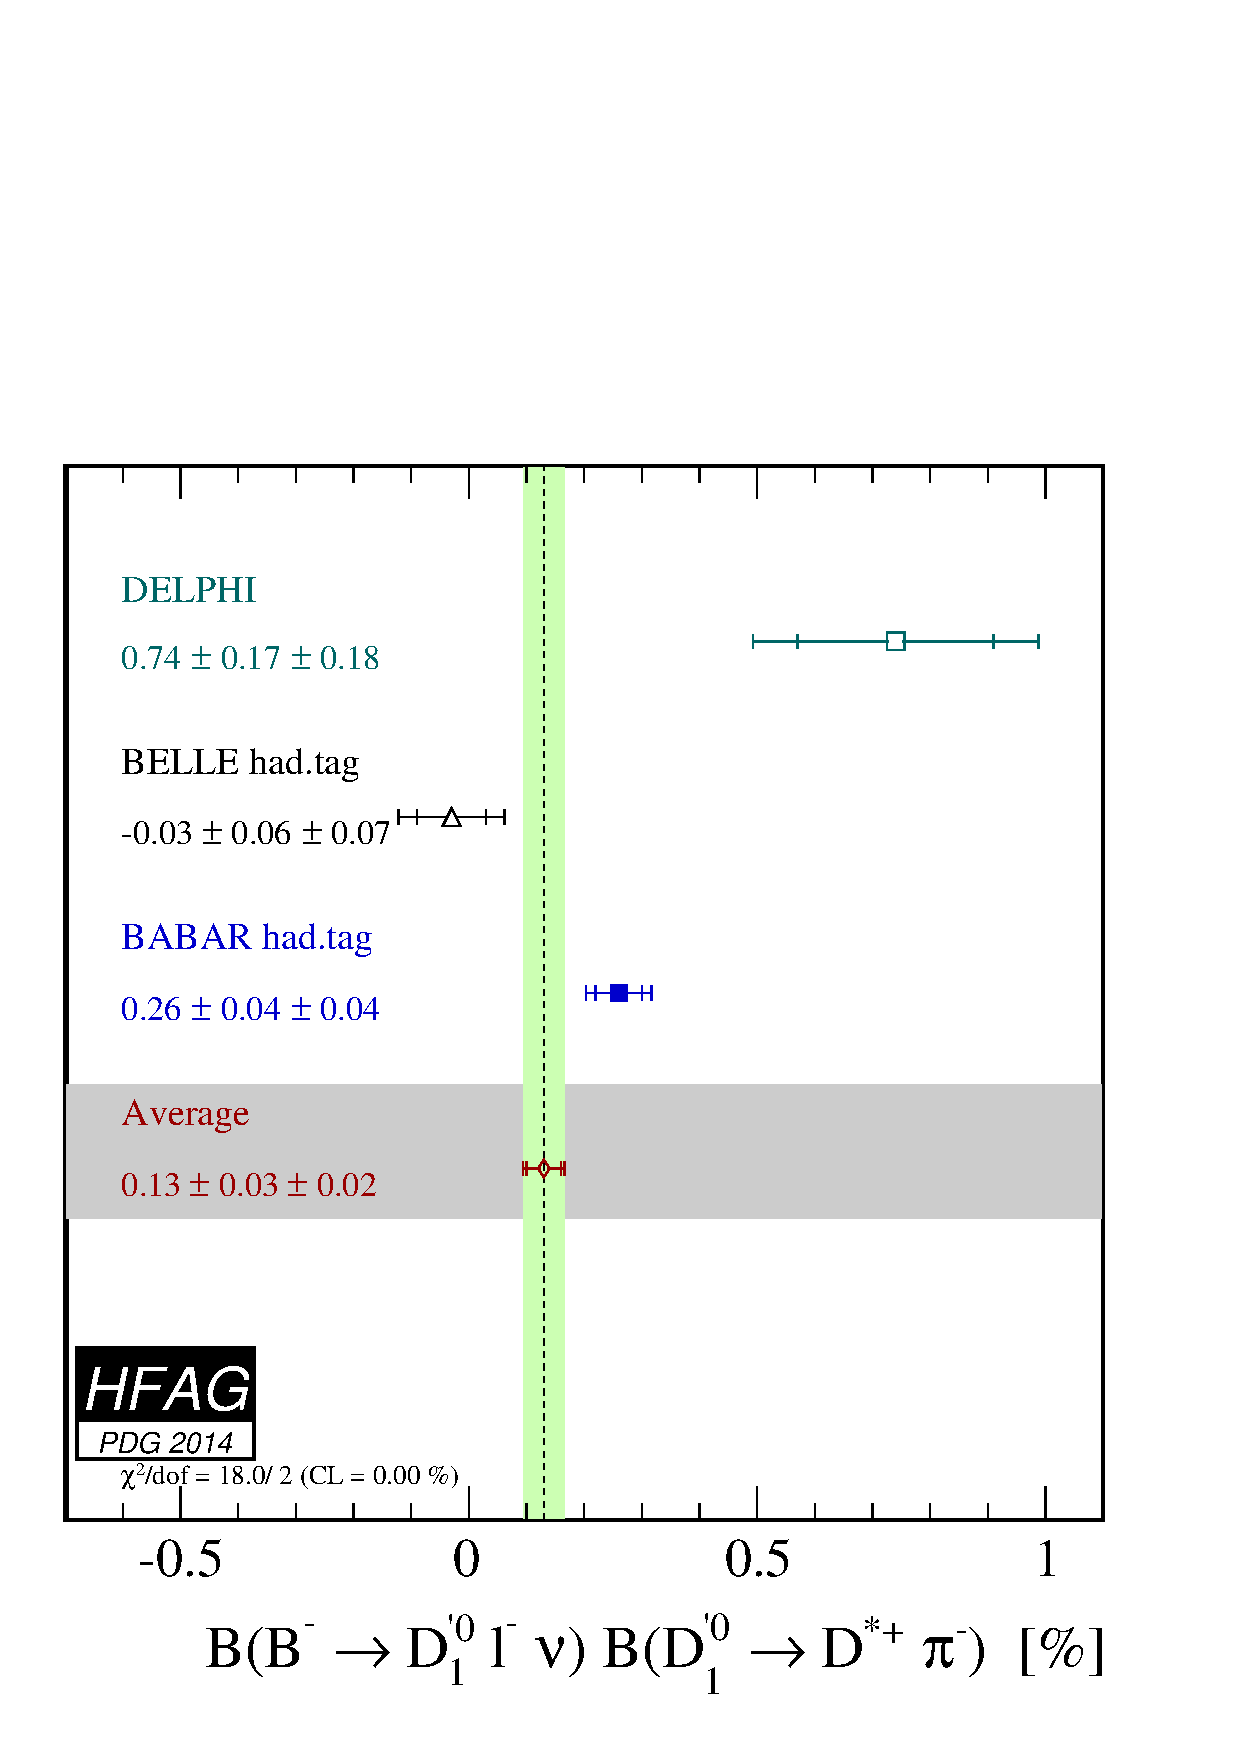
\includegraphics[width=7.8cm]{figures/slb/br_dss1primel.pdf}
   }
   \put(  8.0,  0.0){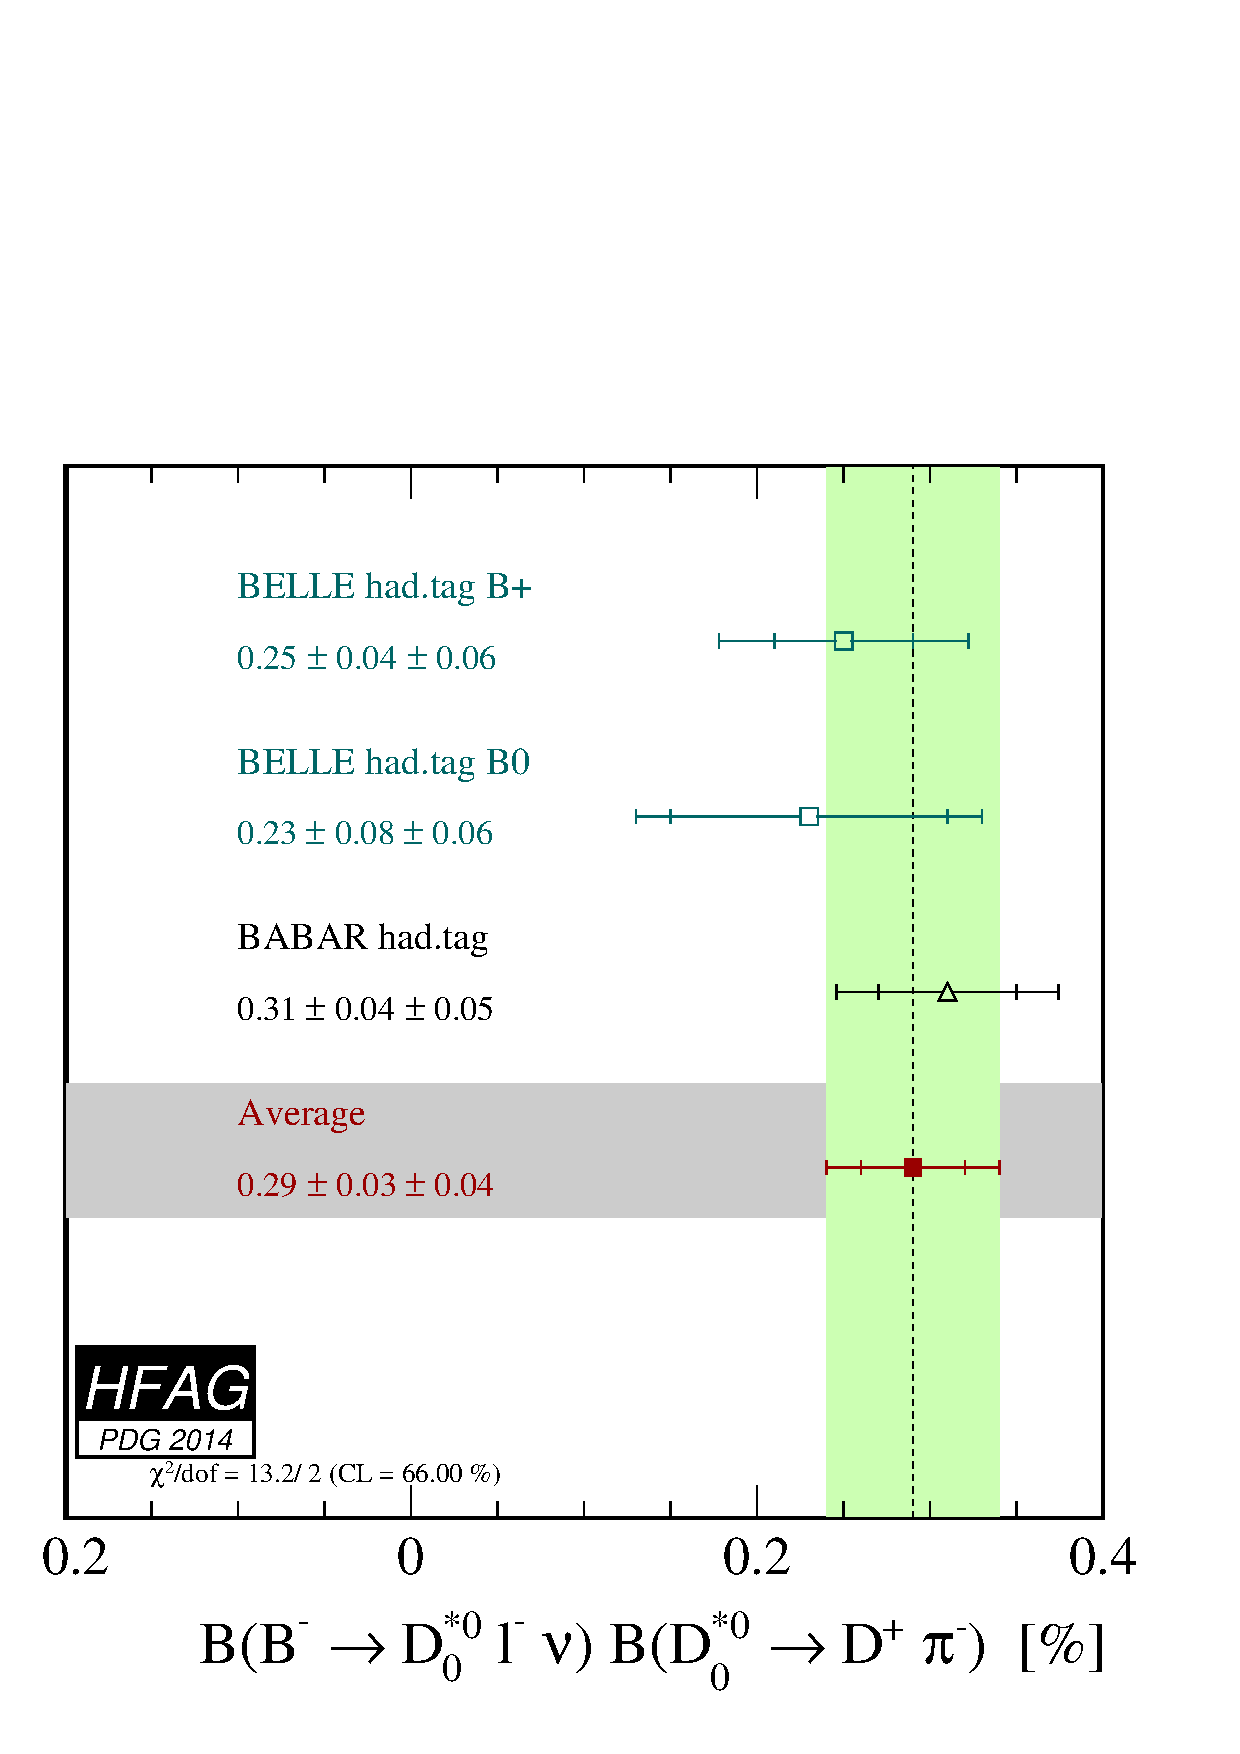
\includegraphics[width=7.8cm]{figures/slb/br_dss00l.pdf}
   }
   \put(  5.5,  7.3){{\large\bf a)}}
   \put( 14.4,  7.3){{\large\bf b)}}
  \end{picture}
  \caption{Average of the product of branching fraction (a) 
  $\cbf(B^- \to D_1'^0(D^{*+}\pi^-)\ell^-\bar{\nu}_{\ell})
\times \cbf(D_1'^0 \to D^{*+}\pi^-)$ and (b) $\cbf(B^- \to D_0^{*0}(D^{*+}\pi^-)\ell^-\bar{\nu}_{\ell})
\times \cbf(D_0^{*0} \to D^{+}\pi^-)$
The corresponding individual
  results are also shown.}
  \label{fig:brdssl2}
 \end{center}
\end{figure}
